% Author: Jannes Bantje
% Modified: Lars Haalck lars.haalck@wwu.de
% please ask Lars Haalck first if you have any questions
%!TEX root = AutoML-fuer-Segmentierung.tex
% Author: Jannes Bantje
% Modified: Lars Haalck lars.haalck@wwu.de
% please ask Lars Haalck first if you have any questions

\documentclass[%
a4paper,
parskip=half,
index=totoc,
toc=listof,
fontsize=11,
headinclude,
twoside,
BCOR=12mm,
cleardoublepage=empty,
DIV=13,
draft=false % delete this line completely to remove all todos
]{scrreprt}


\usepackage{multirow}
\usepackage[usenames,x11names]{xcolor}
\usepackage[final]{graphicx}
\usepackage{subcaption}
\usepackage{float}

% typographic settings, fonts, and math
\usepackage[utf8]{inputenc}
\usepackage[lining,semibold]{libertine}
\usepackage[T1]{fontenc}
\usepackage{textcomp} % verhindert ein paar Fehler bei den Fonts
\usepackage[varl]{zi4}
\usepackage{mathtools,amssymb,amsthm} % Verbesserung von amsmath (die amsmath selbst lädt)
\usepackage[libertine,cmintegrals,bigdelims,varbb]{newtxmath}
\usepackage[ngerman]{babel}
\usepackage[babel=true, tracking=true,final]{microtype}
\usepackage[ngerman]{datetime}



% set line spacing
\usepackage{setspace}
% for example 1.5 line spacing
\onehalfspacing

% literature settings
\usepackage[
backend=biber,
sortlocale=auto,
natbib,
hyperref=true,
backref=false,
mincitenames=1,
maxcitenames=1,
style=ieee
]%
{biblatex}
\addbibresource{literature.bib} % sets literature file

% hyperref settings to make links clickable in PDF
\usepackage[%
hidelinks,
pdfpagelabels,
bookmarksopen=true,
bookmarksnumbered=true,
linkcolor=black,
urlcolor=SkyBlue2,
plainpages=false,
pagebackref,
citecolor=black,
hypertexnames=true,
pdfborderstyle={/S/U},
linkbordercolor=SkyBlue2,
colorlinks=false,
backref=false
]{hyperref}
\hypersetup{final}

% enumeration settings
\usepackage[shortlabels]{enumitem}
\setlist[enumerate,description]{font=\sffamily\bfseries} % makes labels in enumeration bold
\usepackage[german=quotes]{csquotes}

% allows adding of todo notes at the side of the document
\setlength{\marginparwidth}{0.8cm}
\usepackage[obeyDraft,textsize=tiny,textwidth=1.2cm]{todonotes}

% settings for the header and footer
\usepackage[headsepline=1pt]{scrlayer-scrpage}
\pagestyle{scrheadings}
\clearscrheadfoot % clear defaults
\setkomafont{headsepline}{\color{gray}} % adds a gray line under the header

% set section title on the right, and chapter title on the left page in a double page
% document
\automark[section]{chapter}

\rohead{\rightmark} % section title on the right side
\lehead{\scshape\leftmark} % chapter title on the left side an in small caps
\ofoot[\pagemark]{\pagemark} % page marks always on the outer site of the page

% sets page marks and footer and header texts to sans-serif in gray
\renewcommand*{\pnumfont}{\sffamily}
\renewcommand*{\footfont}{\sffamily\color{gray}}
\renewcommand*{\headfont}{\sffamily\color{gray}}

% change the chapter, section and subsection font sizes and spacings a bit for a5 format
% \setlength{\footskip}{1.75\baselineskip} % change the spacing a bit for a5 format
% \RedeclareSectionCommand[%
% afterskip=1\baselineskip,%
% beforeskip=-1\baselineskip]{chapter}

% \setkomafont{chapter}{\LARGE}
% \setkomafont{section}{\Large}
% \setkomafont{subsection}{\large}

% adds a thick gray line after the chapter number
\renewcommand*{\chapterformat}{%
    \thechapter\enskip
    \textcolor{gray!50}{\rule[-\dp\strutbox]{1.5pt}{\baselineskip}}\enskip
}


% math environments
\usepackage{amsthm}
\usepackage{thmtools}
\usepackage{mdframed}
\usepackage{blindtext}
\renewcommand{\listtheoremname}{Übersicht aller Aussagen}

% -- Theoreme als PDF-Lesezeichen
\usepackage{bookmark}
\bookmarksetup{open,numbered}
\makeatletter
\newcommand*{\theorembookmark}{%
    \bookmark[
    dest=\@currentHref,
    rellevel=1,
    keeplevel,
    ]{%
        \thmt@thmname\space\csname the\thmt@envname\endcsname
        \ifx\thmt@shortoptarg\@empty
            \else
                \space(\thmt@shortoptarg)%
            \fi
        }%
    }
\makeatother

% -- Definition der einzelnen Umgebungen
\declaretheoremstyle[%
headfont=\sffamily\bfseries,
notefont=\normalfont\sffamily,
bodyfont=\normalfont,
headformat=\NAME\ \NUMBER\NOTE,
headpunct=,
postheadspace=\newline,
spaceabove=\parsep,spacebelow=\parsep,
%shaded={bgcolor=gray!20},
postheadhook=\theorembookmark,
mdframed={
    backgroundcolor=gray!20,
    linecolor=gray!20,
    innertopmargin=6pt,
    roundcorner=5pt,
    innerbottommargin=6pt,
    skipbelow=\parsep,
skipbelow=\parsep }
]%
{mainstyle}

\declaretheoremstyle[%
headfont=\sffamily\bfseries,
notefont=\normalfont\sffamily,
bodyfont=\normalfont,
headformat=\NAME\ \NUMBER\NOTE,
headpunct=,
postheadspace=\newline,
spaceabove=15pt,spacebelow=10pt,
postheadhook=\theorembookmark]%
{mainstyle_unshaded}

\declaretheoremstyle[%
headfont=\sffamily\bfseries,
notefont=\normalfont\sffamily,
bodyfont=\normalfont,
headformat=\NUMBER\NAME\NOTE,
headpunct=,
postheadspace=\newline,
spaceabove=15pt,spacebelow=10pt,
% shaded={bgcolor=gray!20},
postheadhook=\theorembookmark]%
{mainstyle_unnumbered}

\declaretheorem[name=Definition,parent=section,style=mainstyle]{definition}
\declaretheorem[name=Definition,numbered=no,style=mainstyle]{definition*}
\declaretheorem[name=Definition,sharenumber=definition,style=mainstyle_unshaded]{definitionUnshaded}

\declaretheorem[name=Theorem,sharenumber=definition,style=mainstyle]{theorem}
\declaretheorem[name=Theorem,numbered=no,style=mainstyle_unnumbered]{theorem*}

\declaretheorem[name=Proposition,sharenumber=definition,style=mainstyle]{proposition}
\declaretheorem[name=Lemma,sharenumber=definition,style=mainstyle]{lemma}

\declaretheorem[name=Satz,sharenumber=definition,style=mainstyle]{satz}
\declaretheorem[name=Satz,sharenumber=definition,style=mainstyle_unshaded]{satzUnshaded}
\declaretheorem[name=Satz,numbered=no,style=mainstyle_unnumbered]{satz*}

\declaretheorem[name=Korollar,sharenumber=definition,style=mainstyle]{korollar}

\declaretheorem[name=Notation,numbered=no,style=mainstyle_unnumbered]{notation}
\declaretheorem[name=Bemerkung,numbered=no,style=mainstyle_unnumbered]{bemerkung}
\declaretheorem[name=Beispiel,numbered=no,style=mainstyle_unnumbered]{beispiel}
\declaretheorem[name=Beispiele,numbered=no,style=mainstyle_unnumbered]{beispiele}



%Informationen zur Arbeit
\newcommand{\printname}{
Milan Blunk (418650) \\ 
Pia Nümann (454700) \\
Matthias Wolff (458766)
}
%\newcommand{\printgroup}{Gruppe 01}
%\newcommand{\printnumber}{XXX XXX}

\newcommand{\printtitle}{AutoML für Segmentierung}
\newcommand{\printcity}{Münster}
\newcommand{\printtype}{Projektseminar}
\newcommand{\printdegree}{AutoML}
%\newcommand{\printsupervisor}{John Doe}
%\newcommand{\printfirstassessor}{Prof. Dr. Erika Musterfrau}
%\newcommand{\printsecondassessor}{Prof. Dr. Hans Peter}
\newcommand{\printinstitute}{Institut für Informatik}


\begin{document}
% set the pager numbering to big roman numbers for first few pages
\pagenumbering{Roman}
%\listoftodos

% titlepage does not need cleardoubleoddemptypage
\begin{titlepage}
	\thispagestyle{empty}

\begin{center}
    
\includegraphics[width=7.5cm]{logos/wwu-logo.eps}
    \par
    \vspace*{8ex}
    \LARGE
    \printtitle
    \par
    \normalsize
    \vspace*{8ex}
    \large
    \textsc{\printtype}\\
    \normalsize
    zum Thema\\
    \large
    \textsc{\printdegree}
    \par
    \normalsize
    \vspace*{6ex}
    Westfälische Wilhelms-Universität Münster\\
    \printinstitute
\end{center}

%\par
%\vspace*{6ex}
%Betreuung:\\
%\large
%\textit{\printsupervisor}
%
%\par
%\normalsize
%\vspace*{2ex}
%Erstgutachter:\\
%\large
%\textit{\printfirstassessor}
%
%\par
%\normalsize
%\vspace*{2ex}
%Zweitgutachter:\\
%\large
%\textit{\printsecondassessor}

\vspace*{5cm}
\par
\normalsize
\vspace*{2ex}
Eingereicht von:\\
\large
\textit{\printname}\\
%\textit{\printgroup}

\par
\normalsize
\vspace*{4ex}
\printcity, \makeatletter
\monthname
\makeatother~\the\year

\end{titlepage}

\tableofcontents

% set the page numbering back to arabic
\pagenumbering{arabic}
\setcounter{page}{1}



% Einführung
%!TEX root = ../AutoML-fuer-Segmentierung.tex
\chapter{Einführung}
\label{ch:intro}

Diese Ausarbeitung ist Gegenstand des Projektseminars \enquote{AutoML}, das im Wintersemester 2020/2021 an der Westfälischen Wilhelms Universität unter der Leitung von Prof. Xiaoyi Jiang und Christof Duhme durchgeführt wurde.\\
In dem Projektseminar haben sich neun Teilnehmer zu drei Dreiergruppen zusammengefunden. Die Themen der drei Gruppen waren: \enquote{AutoML Frameworks}, \enquote{AutoML für Segmentierung} und \enquote{NAS ohne Training}.\\
Wir haben uns mit Thema zwei \enquote{AutoML für Segmentierung} beschäftigt und beschreiben im Folgenden unsere Vorgehensweise, Probleme, die wir hatten, Erfolge, die wir erzielen konnten, und gehen zu jedem Framework, das wir genutzt haben, auf die Theorie zu der Architektursuche ein. Insgesamt haben wir uns mit drei Frameworks beschäftigt: NAS-Unet, Auto-DeepLab und nnU-Net. Die Arbeit ist so aufgebaut, dass wir jedem Framework ein Kapitel widmen, in dem wir erst jeweils die Theorie erklären, anschließend von unserer Vorgehensweise mit dem Framework berichten, dann die Ergebnisse einordnen und bewerten und abschließend ein Fazit ziehen. Im Anschluss an diese Einführung werden wir so also in Kapitel 2 über NAS-Unet berichten, Kapitel 3 befasst sich mit Auto-DeepLab, anschließend gehen wir auf das nnU-Net ein, mit welchem wir die mit Abstand besten Erfolge erzielen konnten, wie wir in Kapitel 4 sehen werden, ehe wir in Kapitel 5 ein Gesamtfazit ziehen.\\
Zu jedem Framework haben wir das Ziel verfolgt, die Theorie zu verstehen und das Framework anhand verschiedener Datensätze zu testen und zu bewerten. Die Kapitel spiegelen in ihrer Reihenfolge auch die Reihenfolge wieder, in der wir uns mit den verschiedenen Programmen beschäftigt haben. So haben wir mit NAS-Unet angefangen. Zunächst haben wir versucht, auf unseren eigenen Geräten zu arbeiten. Wir mussten jedoch schnell feststellen, dass NAS-Unet auf Windows nicht unterstützt wird und auf MacOS fehlte uns eine Grafikkarte für die Ausführung. Deswegen haben wir an unseren Windows-Geräten eine Linux Distribution installiert. Doch auch so konnten wir nicht zufriedenstellend arbeiten, da die Architektursuche zu aufwendig ist für unsere Geräte.\\ So haben wir glücklicherweise die Möglichkeit bekommen auf den Universitäts-Servern zu arbeiten. All unser Vorgehen haben wir so auf PALMA II (kurz für \enquote{Paralleles Linux-System für Münsteraner Anwender} \cite{palmaII}) ausgeführt. PALMA II ist ein \enquote{Computercluster mit über 18.000 Prozessorkernen, deren Zusammenwirken auch die Lösung komplexester Aufgaben aus Wissenschaft und Forschung ermöglicht.} \cite{palmaII}. So hatten wir leistungsstarke Hardware zur Verfügung, auf denen wir die komplexen Berechnungen ausführen konnten.\\
Nachdem die technischen Rahmenbedingungen nun auch erklärt sind, sei noch zu erwähnen, dass dieser Bericht ein (fundiertes) Grundwissen im Bereich Machine Learning voraussetzt.

%Hier kann beliebig \section{} gesetzt werden

% Einträge in die ToDo-Liste setzen (für Änderungen muss 2 mal übersetzt werden, wie bei TOC auch)






% NAS-Unet
%!TEX root = ../AutoML-fuer-Segmentierung.tex
\chapter{NAS-Unet}
\label{ch:nasunet}


% Einträge in die ToDo-Liste setzen (für Änderungen muss 2 mal übersetzt werden, wie bei TOC auch)
\todo{NAS-Unet mit Inhalt füllen}


\section{Funktionsweise / Theorie}


NAS-Unet ist einer der ersten Versuche NAS auf medizinische Bildsegmentierung anzuwenden. Es sollten MRT-, CT- und Ultraschallbilder segmentiert werden. Die Architektur von NAS-Unet wurde auf Pascal VOC2012 \cite{PascalVOCDatensatz} gesucht und diese dann auf den unterschiedlichen medizinischen Datensätzen trainiert. Als medizinische Datensätze werden für die MRT-Bilder der Promise12 Datensatz \cite{Promise12Datensatz}, für die CT-Bilder der Chaos Datensatz \cite{ChaosDatensatz} und für die Ultraschallbilder der NERVE Datensatz \cite{NerveDatensatz} verwendet. 

Das vorrangige Ziel von NAS-Unet ist das automatische Finden einer geeigneten Zwei-Zell Architektur. Dabei wird parallel nach der Up-Sampling und nach der Down-Sampling Schicht gesucht, die beiden Schichten werden gleichzeitig upgedated. Dabei wird also immer eine Up-Sampling Zelle gleichzeitig mit der ihr gegenüberliegenden Down-Sampling Zelle aktualisiert. Die Architektur von NAS-Unet ist streng symmetrisch und es gibt keine zusätzliche Convolutionschicht in der Mitte (siehe Abbildung \ref{pic:nasUnet_ArchitekturGesamt}). 

\begin{figure}[H]
	
	\centering
	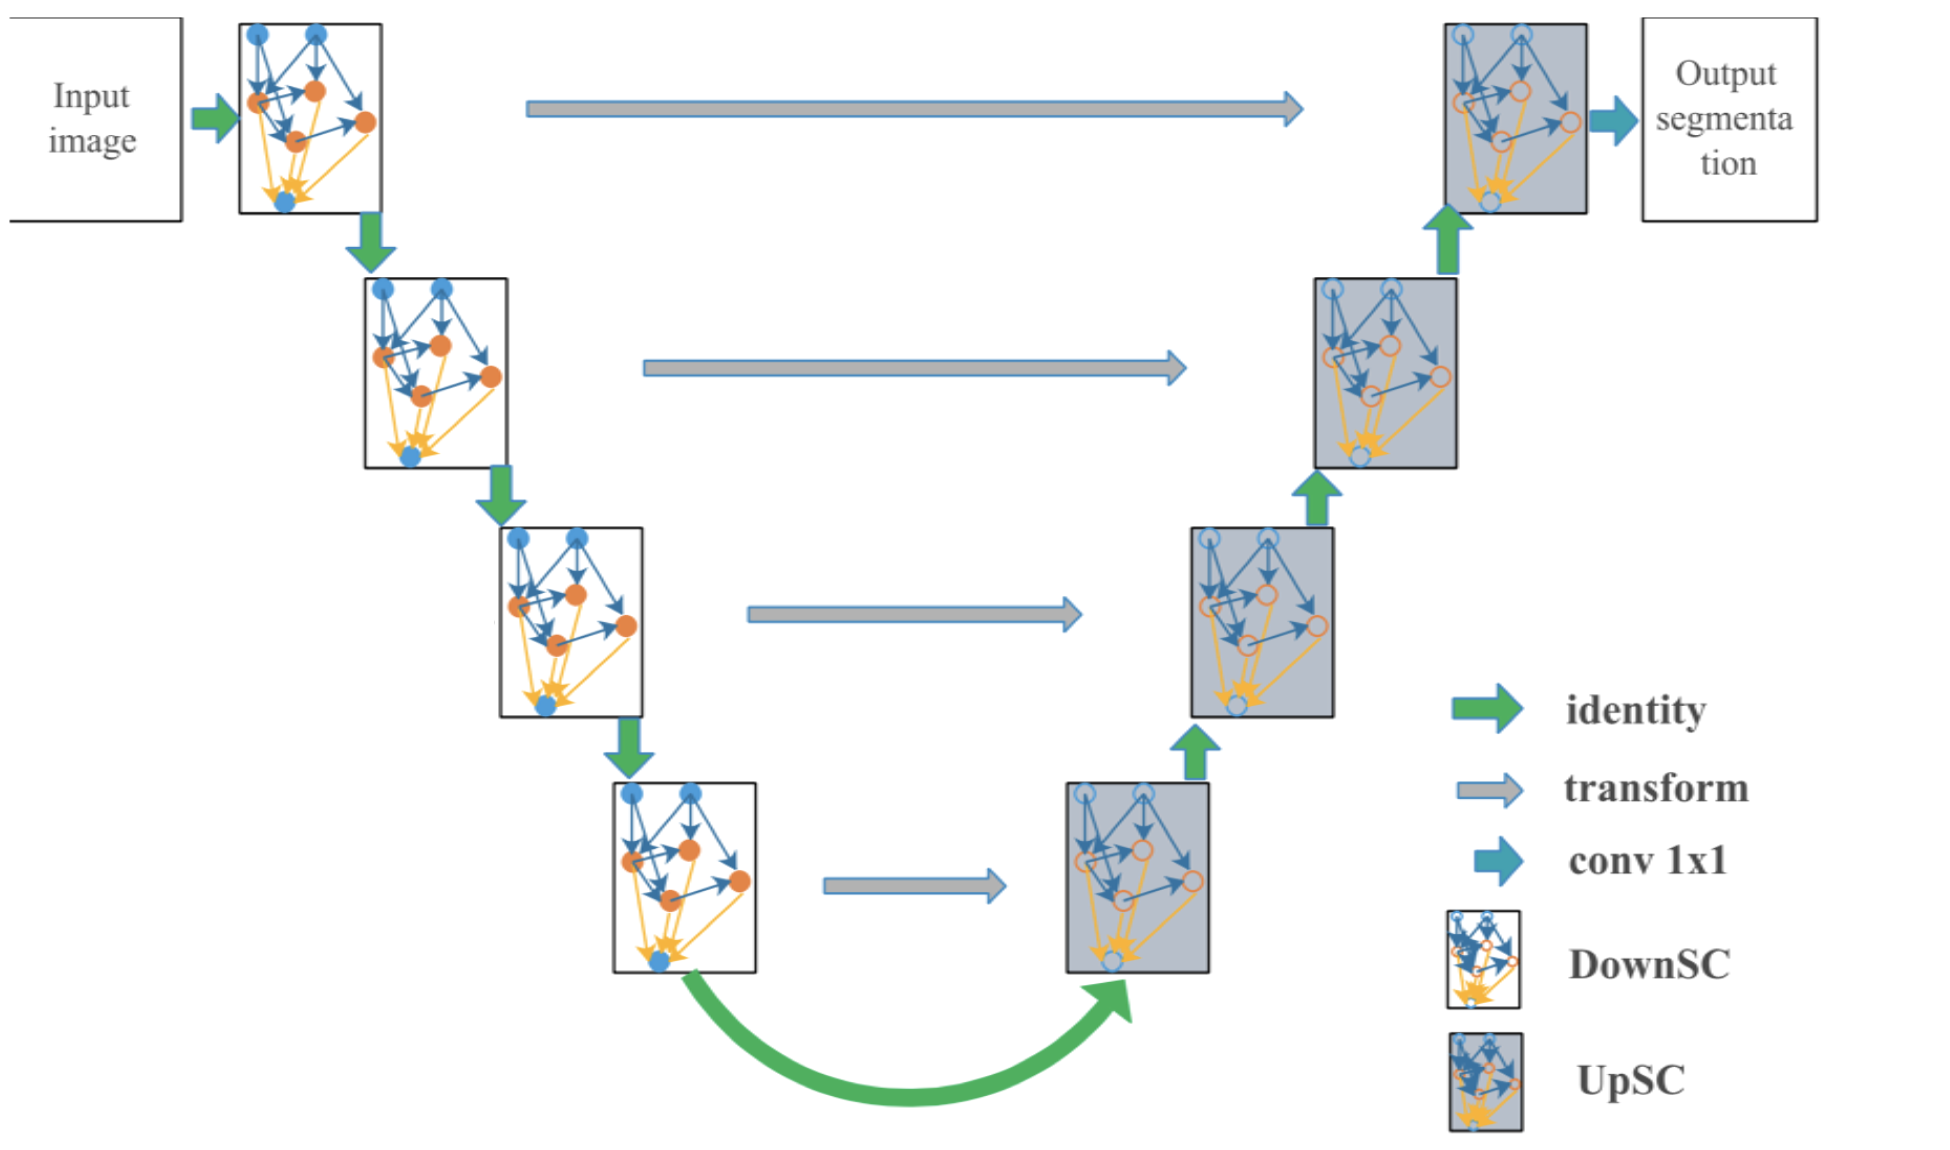
\includegraphics[scale=0.5]{Pictures/nasUnet/Bild1.png}
	\caption{Zellbasierte Netzarchitektur von NAS-Unet \cite{nasunetPaper} }
	\label{pic:nasUnet_ArchitekturGesamt}
\end{figure}

Der Suchraum, in dem die Architektur gesucht werden soll, enthält die möglichen Architekturen die prinzipiell verwendet werden können, sowie eine Auswahl von primitiven Operationen. Die möglichen Architekturen sind populäre Unet-Architekturen, von denen nur die mittlere Convolutionschicht entfernt wurde. 
NAS-Unet verwendet einen zell-basierten Architektursuchraum. Die zell-basierte Architektur (siehe Abbildung \ref{pic:nasUnet_ArchitekturGesamt}) soll die Generierungsmethode beschränken und so das Problem lösen, dass der Suchraum zu groß wird. Nachdem die beste Zellarchitektur (siehe Abbildung \ref{pic:nasUnet_Zellarchitektur}) gefunden wurde, wird sie im ganzen Netzwerk genutzt und im Rückrad des Netzes gestapelt. Dabei sind nicht nur die Convolutionschichten in die Zellen verlegt, sondern auch alle Up- und Down-sampling Operationen. Die Inputknoten einer Schicht sind definiert als die Outputknoten der vorherigen zwei Schichten (siehe Abbildung \ref{pic:nasUnet_Zellarchitektur}). 
Bei der Auswahl der primitiven Operatoren wurde zum einen darauf geachtet Redundanz zu vermeiden und zum anderen darauf, möglichst wenige Parameter zu haben, um möglichst wenig Memory zu verbrauchen. 

\begin{figure}[H]
	
	\centering
	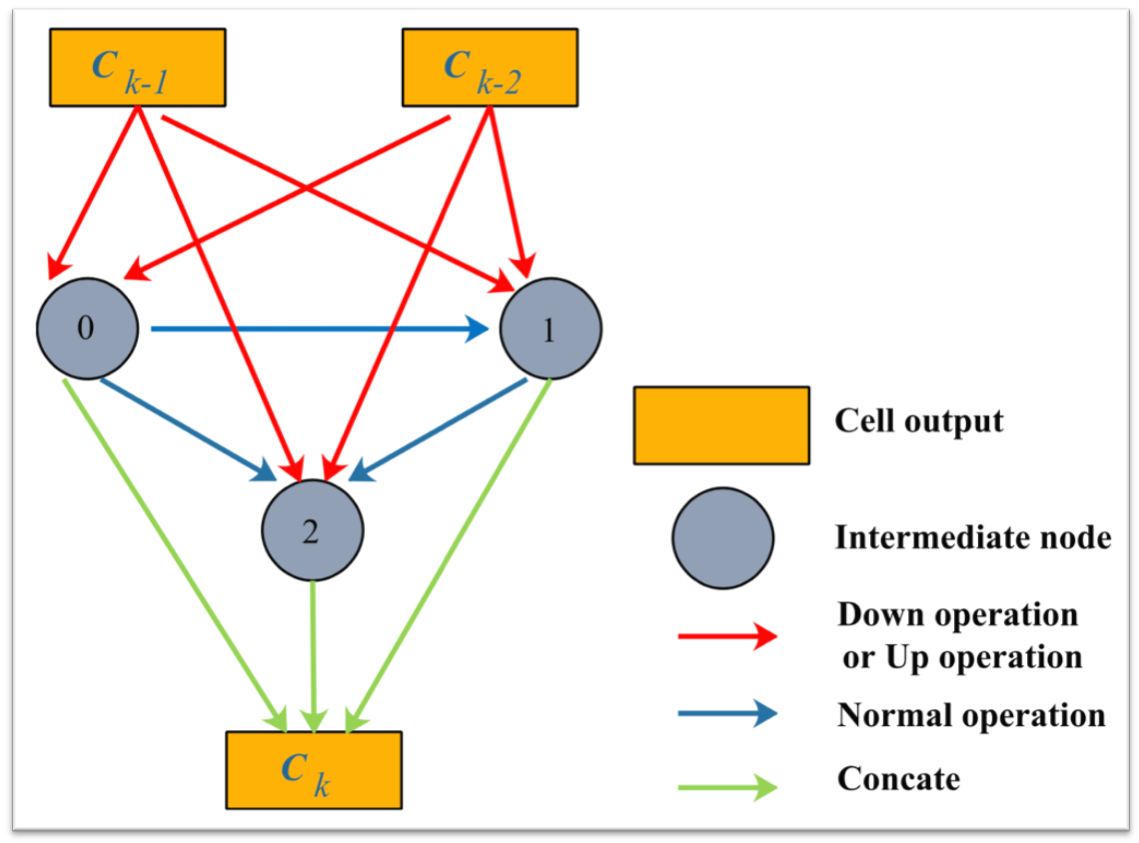
\includegraphics[scale=0.39]{Pictures/nasUnet/Bild2.png}
	\caption{Zellarchitektur von NAS-Unet \cite{nasunetPaper} }
	\label{pic:nasUnet_Zellarchitektur}
\end{figure}

Die Suchstrategie teilt sich in mehrere Schritte auf. Zunächst wird ein überparametrisiertes Netzwerk erstellt (Siehe Abbildung \ref{pic:nasUnet_Zellarchitektur_überparametrisiert}).

\begin{figure}[H]
	
	\centering
	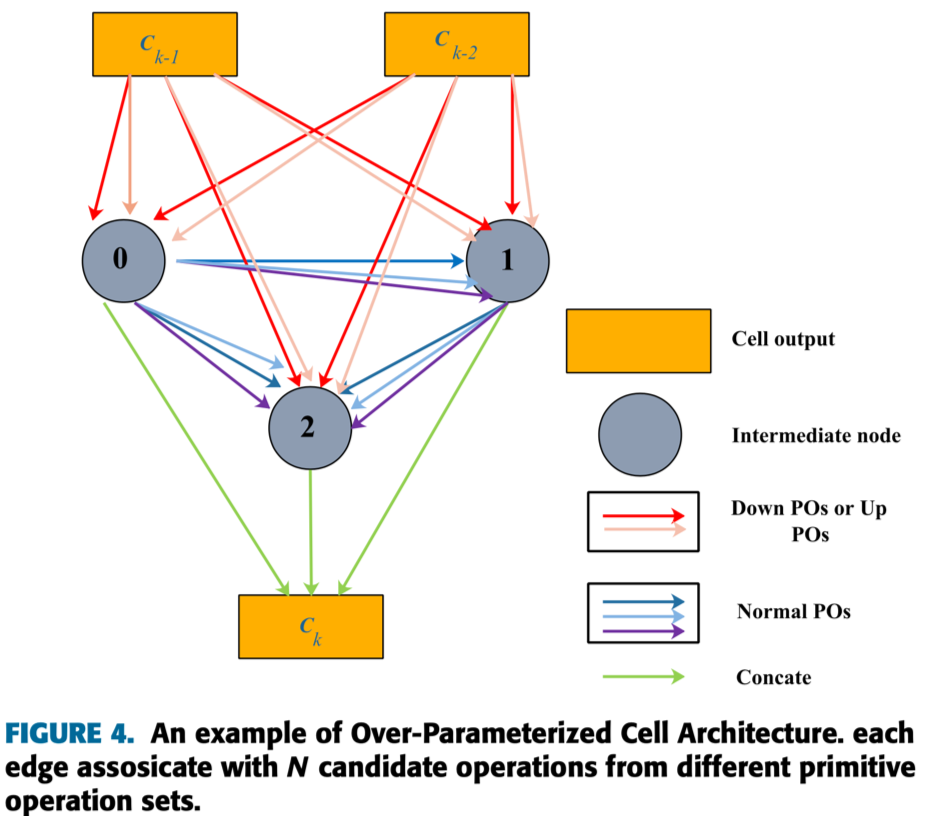
\includegraphics[scale=0.5]{Pictures/nasUnet/Bild3.png}
	\caption{überparametrisierte Zellarchitektur von NAS-Unet \cite{nasunetPaper} }
	\label{pic:nasUnet_Zellarchitektur_überparametrisiert}
\end{figure}


In diesem überparametrisierten Netzwerk lässt sich der Output einer Kante aus der Kombinationen der unterschiedlichen primitiven Operatoren folgendermaßen als Formel darstellen: $$MixO(x)=\sum\limits_{i=1}^{N}w\textsubscript{i}o\textsubscript{i}(x)$$
Dabei ist o(x) die Primitive Operation, w ist das zu der Operation gehörende Gewicht und N ist die Anzahl an primitieven Operationen. 

Um die Parameter zu aktualisieren, wird eine effizienter Parameter-Update Strategie verwendet, damit GPU-Memory gespart wird. Da die Output-Feature-Maps nur berechnet werden können, wenn alle Operationen gleichzeitig im GPU-Memory sind, wird das N-fache an GPU-Memory benötigt, als wenn man ein kompaktes Modell trainieren würde. Daher wird hier ein binärer Ansatz verwendet, das heißt anstatt bei jedem Schritt alle Architekturparameter mit dem Gradientenabstiegsverfahren zu aktualisieren, wird immer nur ein Parameter aktualisiert (siehe Abbildung \ref{pic:nasUnet_binäreSuchstrategie}). Dadurch werden aber mehr Iterationen des Updatens benötigt.

\begin{figure}[H]
	
	\centering
	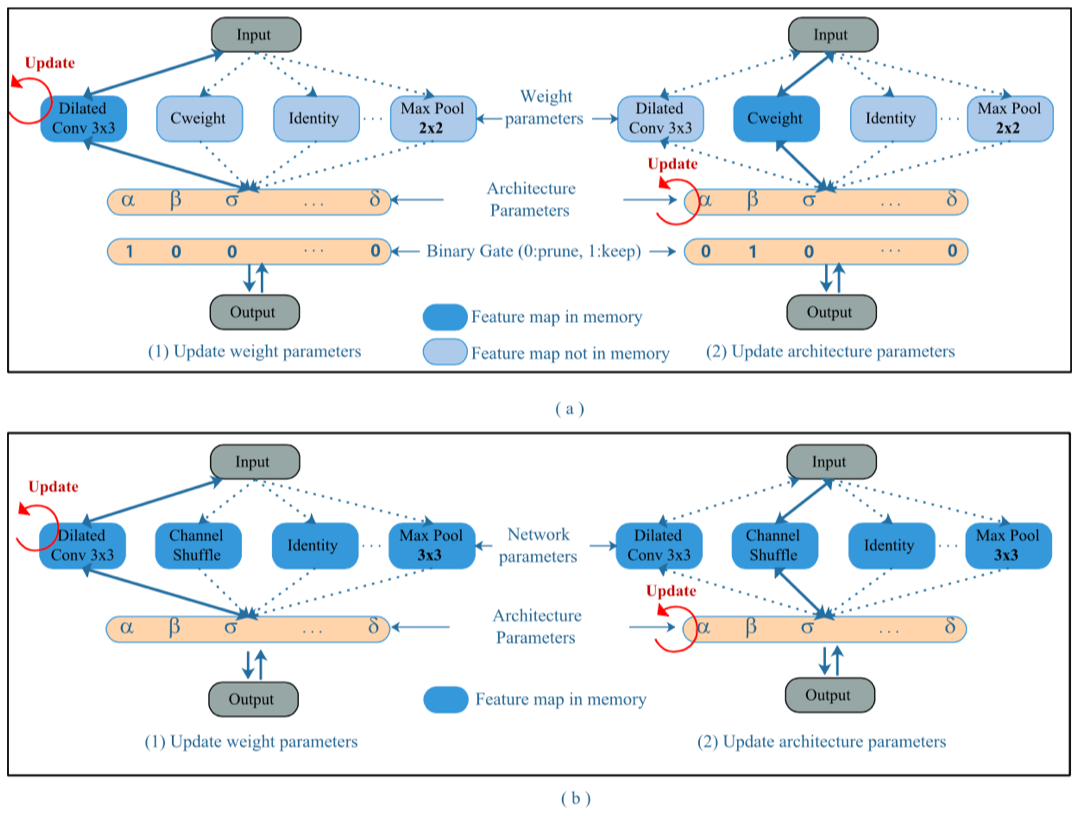
\includegraphics[scale=0.7]{Pictures/nasUnet/Bild4.png}
	\caption{Vergleich der binären Suchstrategie von NAS-Unet mit dem gleichzeitigen Updaten aller Parameter \cite{nasunetPaper} }
	\label{pic:nasUnet_binäreSuchstrategie}
\end{figure}

Zu den Implemetierungsdetails gehört, dass es immer jeweils 4 Up- und Downsampling Zellen gibt. Die Bilder werden zufällig zur einen Hälfte in Trainingsbilder und zur anderen Hälfte in Testbilder eingeteilt. 
Das Paper konzentriert sich vorrangig darauf einen effizienten Suchraum zu konstruieren. Die Suchstrategie ist für die Autoren weniger wichtig, da laut ihrer Aussage (Paper, II. B. \cite{nasunetPaper} und Page 44253, Satz2, \cite{nasunetPaper}) jede differentielle Suchstrategie auf dem Suchraum funtionieren würde. In diesem konkreten Fall wird die DARTS-Update Strategie verwendet. 

\section{Unsere Arbeit / Praxis}

Bei der praktischen Arbeit mit NAS-Unet sind wir auf verschiedene Schwierigkeiten und Hindernisse gestoßen. Diese belaufen sich vorranging auf die Problematik, dass es keine Anleitung oder Einführung für Nas-Unet gibt und auch nahezu keine Dokumentation vorliegt. 
Zunächst einmal haben wir versucht NAS-Unet auf verschiedenen Datensätzen zum Laufen zu bekommen. Dies waren der Datensatz Pascal VOC, der Chaos Datensatz und der Promise Datensatz, welche alle auch im Paper verwendet werden. Bereits hier hatten wie einige Schwierigkeiten, die wir zum Teil auch nicht überwinden konnten. 

Als erstes haben wir durch Fehlermeldungen und Suchen im Code herausgefunden, dass NAS-Unet den Datensatz in einem ganz bestimmten Ordner an einem ganz bestimmten Pfad erwartet. Da wir den Pfad auf Palma nicht einrichten konnten, da dieser schon im Wurzelverzeichnis beginnt, mussten wir die Stelle im Code entsprechend anpassen. Die Tatsache, dass der Code fast gar nicht kommentiert wurde, hat uns die Suche und Anpassung erheblich erschwert. Auch die Ordnernamen und die Struktur des Datensatzes mussten angepasst werden. Auch hierzu gab es keinerlei Hinweise oder Dokumentation. 

Auf dem Chaos Datensatz, welcher auch im Paper verwendet wird, hatten wir das Problem, dass das Framework im Datensatz nach Bildern sucht, die in keiner öffentlich verfügbaren Version des Datensatzes \cite{ChaosDatensatz} existieren. Wie das NAS-Unet auf diese Bilder kommt oder wie man verhindert, dass es nach diesen sucht, ist uns unklar geblieben. 

Während wir den Promise Datensatz nicht öffentlich zugänglich finden konnten, ließ sich das Framework auf dem Pascal VOC Datensatz erfolgreich ausführen. 


\section{Ergebnisse}

Erfolgreich zum Laufen bringen konnten wir das Netz lediglich auf dem Datensatz Pascal VOC2012. Unsere erzielten Ergebnisse waren jedoch leider sehr schlecht. Unsere mIoU auf dem Pascal Datensatz auf den Testbildern war <0.05 (siehe Abbildung \ref{pic:nasUnet_Ergebnisse}). 

\begin{figure}[H]
	
	\centering
	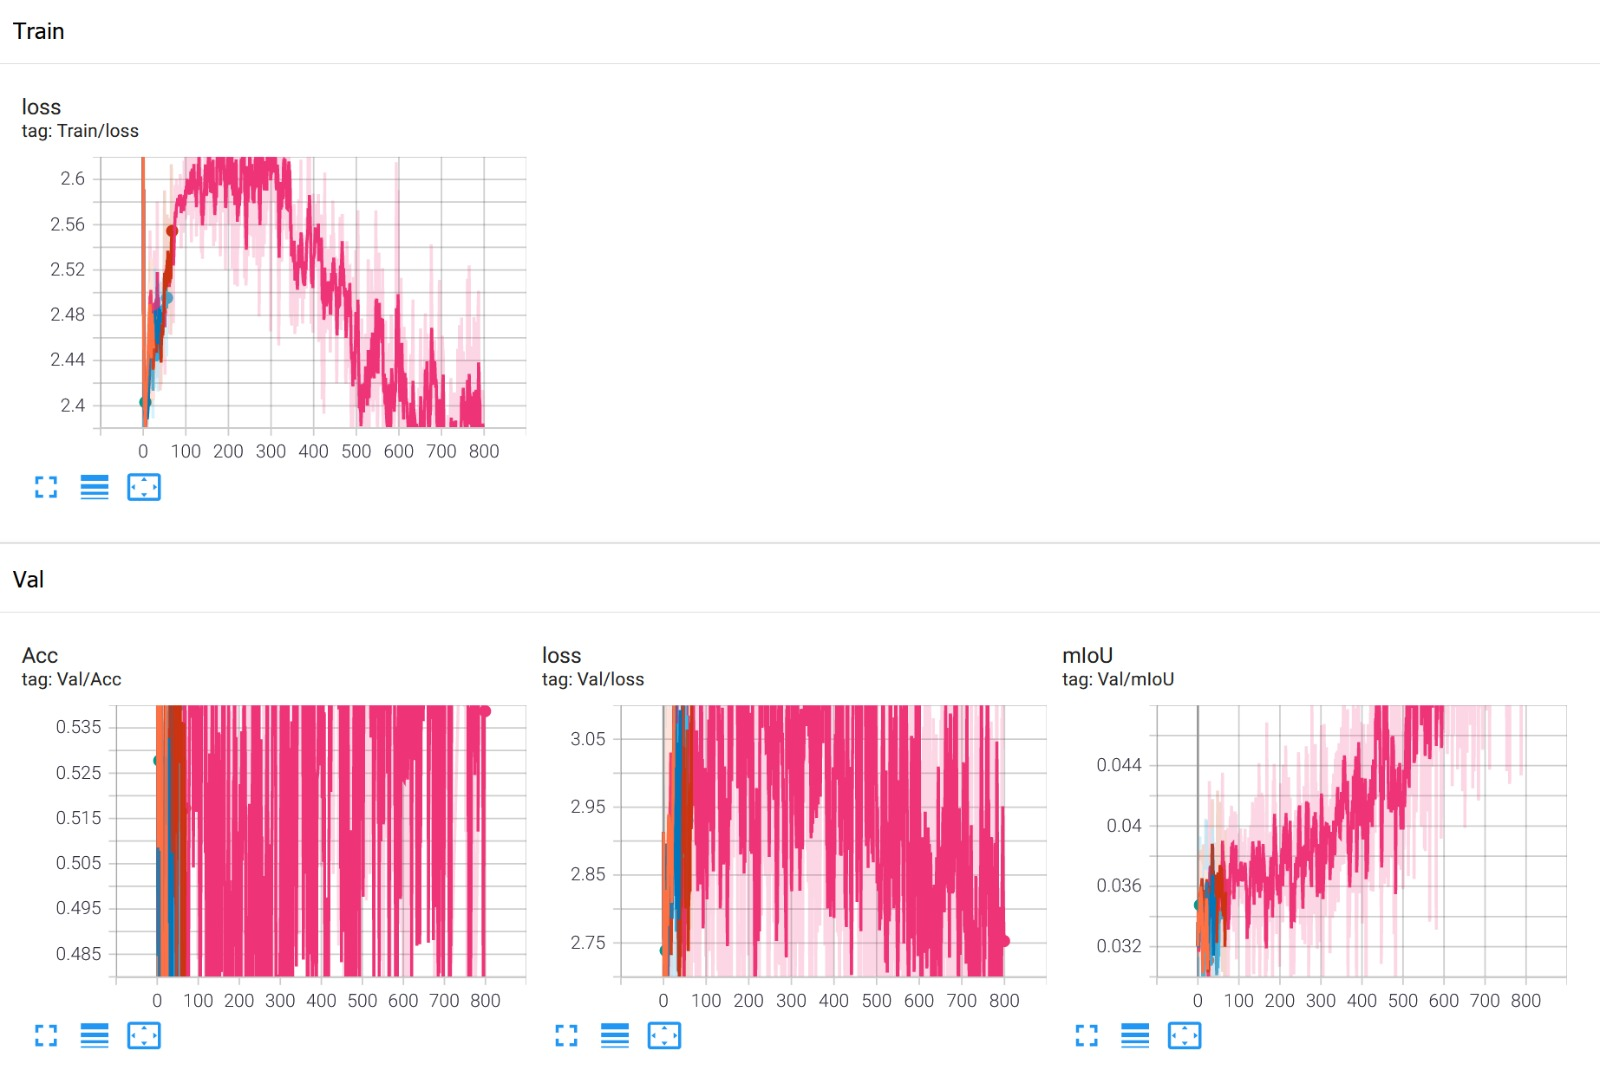
\includegraphics[scale=0.25]{Pictures/nasUnet/Bild5.png}
	\caption{überparametrisierte Zellarchitektur von NAS-Unet \cite{nasunetPaper} }
	\label{pic:nasUnet_Ergebnisse}
\end{figure}

Wie man sieht, ist der Graphenverlauf sehr schwankend und ergibt nur stark gesmoothed eine sichtbare Tendenz. Die Werte sind schlecht bis sehr schlecht, und verbessern sich auch nur sehr langsam.

Auf dem Chaos-Datensatz haben wir NAS-Unet nicht zum Laufen bekommen, da NAS-Unet nach einem Bild sucht, welches in keiner der öffentlichen Versionen des Datensatzes (\cite{ChaosDatensatz} unter Download) existiert. Da es uns nicht gelungen ist, dieses Problem zu lösen, haben wir das Framework leider nicht auf dem Chaos-Datensatz zum Laufen bekommen und können daher auch keine Ergebnisse vorstellen. Uns ist auch nach langer Fehlersuche nicht klar geworden, warum das Framework überhaupt nach einem Bild sucht, welches es eigentlich nie eingegeben bekommen hat. 

Da wir den Promise Datensatz nicht öffentlich finden konnten, können wir hier leider auch über keine Ergebnisse berichten.


\section{Fazit}

Durch die fehlende Dokumentation des Codes und die fehlende Anleitung zur Nutzung des Frameworks ist es extrem schwierig und zeitaufwändig das Framework zu nutzen. Es war uns leider auch nicht möglich, den Code vollständig nachzuvollziehen. Wir konnten daher leider nicht nachvollziehen, was genau gemacht wurde. Auch im Internet, zum Beispiel auf Github, konnten wir leider niemanden finden, der den Code nachvollziehen konnte. Man findet auch hier leider nur viele Fragen. Ein Beispiel ist der folgende Versuch den Code nachzuvollziehen: Fraunhofer siehe Abbildung \ref{pic:nasUnet_FrauenhoferScreenshot} Hier sieht man, dass sich auch die Frage der verschiedenen Metriken auftut. Auch darauf haben wir keine Antwort finden können.

\begin{figure}[H]
	
	\centering
	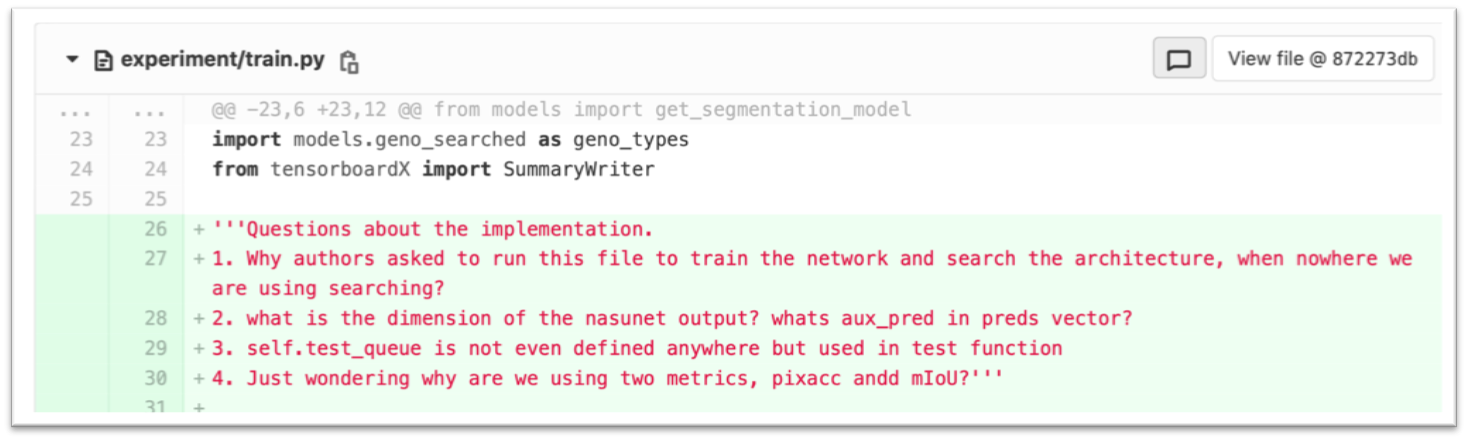
\includegraphics[scale=0.6]{Pictures/nasUnet/Bild6.png}
	\caption{Beispielversuch den Code nachzuvollziehen \cite{Frauenhofer_NasUnet} }
	\label{pic:nasUnet_FrauenhoferScreenshot}
\end{figure}

Ein weiteres Problem ist das Verhalten von NAS-Unet auf dem Chaos Datensatz. Die Frage, warum es nach einem Bild sucht, welches im Datensatz nicht vorkommt, bleibt offen und damit auch die Frage, wie man NAS-Unet auf diesem Datensatz zum Laufen bekommen könnte. Auffällig ist dies vor allem daher, dass NAS-Unet im Paper auch angeblich auf dem Chaos Datensatz angewendet wird. Hier ist wiederum auffällig, dass das Paper zu NAS-Unet am 04.04.2019 veröffentlich wurde, während der Datensatz erst am 11.04.2019 veröffentlich wurde. Möglicherweise hatte die Autoren eine leicht andere Vorversion. Trotzdem erklärt dies nicht, warum das Netz nach mehr Bildern sucht, als ihm eingegeben werden.

Zu den oben genannten Problemen bei der Arbeit mit dem Framework kommt hinzu, dass unsere Ergebnisse auf dem Datensatz Pascal VOC2012 sehr schlecht waren. Besonders auffällig ist dies auf dem Datensatz von Pascal VOC2012, da dieser auch im Paper genutzt wurde und es darauf spezialisiert ist. Leider wurden unserer Recherche nach nie fertig trainierte Modelle von NAS-Unet, welche Ergebnisse wie im Paper angegeben erzielen, veröffentlicht. Daher war es uns leider weder möglich die Ergebnisse zu reproduzieren noch sie nachzuvollziehen.

Im folgenden Github Issue: Issue11 \cite{nasunetGithubIssue11} haben wir herausgefunden, dass man die trainierte Netzstruktur anscheinend händisch in den Code zum Trainieren hineinkopieren muss. Per default verwendet NAS-Unet aber die auf Pascal VOC2012 ausgesuchte Netzstruktur. Daher sollten unsere Ergebnisse auf Pascal VOC 2012 eigentlich davon nicht negativ beeinflusst werden.

Auch beim Durchsuchen der Github Issues auf der zugehörigen Github Seite \cite{nasunetGithub}  sind wir mehrfach darauf gestoßen, dass die Ergebnisse, die im Paper angegeben wurden, nicht reproduziert werden konnten(zum Beispiel Issue 31 \cite{nasunetGithubIssue31}). Da wir auch nicht genau nachvollziehen können, wie diese Ergebnisse entstehen, haben wir uns, auch auf Grund der oben genannten Probleme, dazu entschlossen, nicht länger mit diesem Framework zu arbeiten. Anstelle von NAS-Unet haben wir uns selbstständig ein neues Framework rausgesucht und mit ihm weitergearbeitet (siehe nnU-Net, Kapitel \ref{ch:nnunet}). 





% Deeplab
%!TEX root = ../AutoML-fuer-Segmentierung.tex
\chapter{Deeplab}
\label{ch:deeplab}


% Einträge in die ToDo-Liste setzen (für Änderungen muss 2 mal übersetzt werden, wie bei TOC auch)
\todo{Deeplab mit Inhalt füllen}

\section{Funktionsweise / Theorie}


\section{Unsere Arbeit / Praxis}


\section{Ergebnisse}


\section{Fazit}



% nnUNet
%!TEX root = ../AutoML-fuer-Segmentierung.tex
\chapter{nnUNet}
\label{ch:nnunet}


\section{Funktionsweise / Theorie}



Das nnU-Net ist ein Framework, welches sich mit der Segmentierung von medizinischen 3D-Aufnahmen mit Hilfe von automatisiertem maschinellem Lernen beschäftigt. Es wurde im Rahmen des Medical Segmentation Decathlon Wettbewerb entwickelt und gewann diesen sowie im Anschluss auch viele weitere Segmentierungs-Wettbewerbe. \\
Das nnU-Net verwendet eine klassische und nicht neue U-Net Architektur (not new U-Net). Es konzentriert sich kaum auf  Architekturdesign und -suche, sondern vorrangig auf die Suche von guten Hyperparametern. Es wird eine gleiche oder sehr ähnliche U-Net Struktur immer durch eine individuell auf die individuellen Daten angepasste Trainingspipeline zur Optimierung geschickt (siehe Abbildung \ref{pic:nnUnet_Basisschema}). Das Training der Parameter des Netzes ist also individuell zugeschnitten, während die Architektur sich bei unterschiedlichen Daten nicht oder kaum unterscheidet. Es wird sich also vorrangig auf das Training des Netzes und die Suche individueller Hyperparameter für die Trainingspipeline konzentriert und nicht auf die Suche nach der Architektur. 

\begin{figure}[H]
	
	\centering
	
\includegraphics[scale=0.3]{Pictures/nnUnet/Bild01.png}
	\caption{}
	\label{pic:nnUnet_Basisschema}
\end{figure}



Das nnU-Net verwendet 3 Standardarchitekturen, welche 2D U-Net, 3D full resolution U-Net und 3D U-Net Cascade sind. Vor dem Training kann man einstellen, wie viele und welche Architekturen man trainieren möchte. Per default trainiert nnU-Net alle und wählt am Ende die beste oder die beste Kombination aus maximal zwei Architekturen aus. 2D U-Net eignet sich besonders für 2D-Daten und läuft gut auf anisotropen Daten. Es arbeitet auf den Bildern in Originalauflösung. 3D full resolution U-Net eignet sich für kleine 3D-Daten und arbeitet auch auf den Bildern in Originalauflösung. Bei größeren Bildern werden jedoch die Patches sehr klein, was zum immer größer werdenden Verlust von Kontextdaten führt. Daher gibt es das 3D U-Net Cascade für große 3D-Daten. Es besteht aus 2 hintereinander gereihten U-Nets. Das erste U-Net arbeitet auf den Bildernals ganzes, also ohne Aufteilung in Patches, in geringerer Auflösung. Diese grobe Vorsegmentierung wird zusammen mit dem Bild in Originalgröße an das zweite U-Net weitergegeben. Dieses arbeitet dann wieder auf der vollen Bildauflösung und mit Patches und erstellt eine endgültige und verfeinerte Segmentierung. Durch diesen Übergabeschritt zwischen den beiden U-Nets bleiben die Kontextdaten erhalten (siehe Abbildung \ref{pic:nnUnet_Cascade}).

\begin{figure}[H]
	
	\centering
	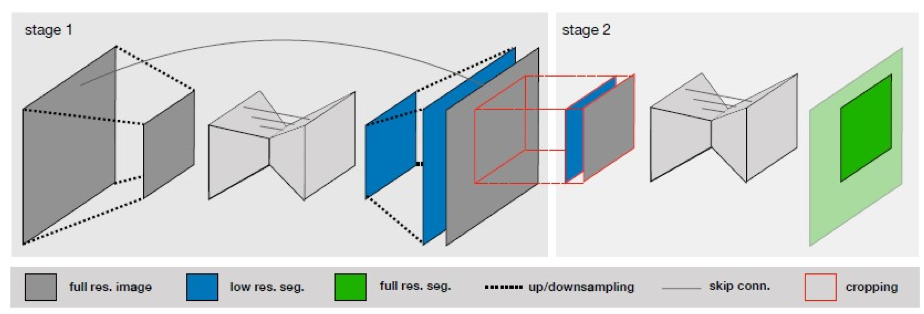
\includegraphics[scale=0.8]{Pictures/nnUnet/Bild02.png}
	\caption{nnU-Net Cascade \cite{nnunetPaper} }
	\label{pic:nnUnet_Cascade}
\end{figure}


Um die Konzentration auf die Anpassung der Hyperparameter der Trainingspipeline an den individuellen Datensatz zu erreichen, wird zunächst ein Datafingerprint aus den Eigenschaften der Trainingsdaten erstellt (siehe Abbildung \ref{pic:nnUnet_Datafingerprint}). Die hierbei genutzten Eigenschaften sind unter anderem die Imgasize, das Pixelvolumen oder die Farbkanäle, die spacing Anisotropie sowie die Anzahl der Klassen und deren Häufigkeitsverteilung. 

\begin{figure}[H]
	
	\centering
	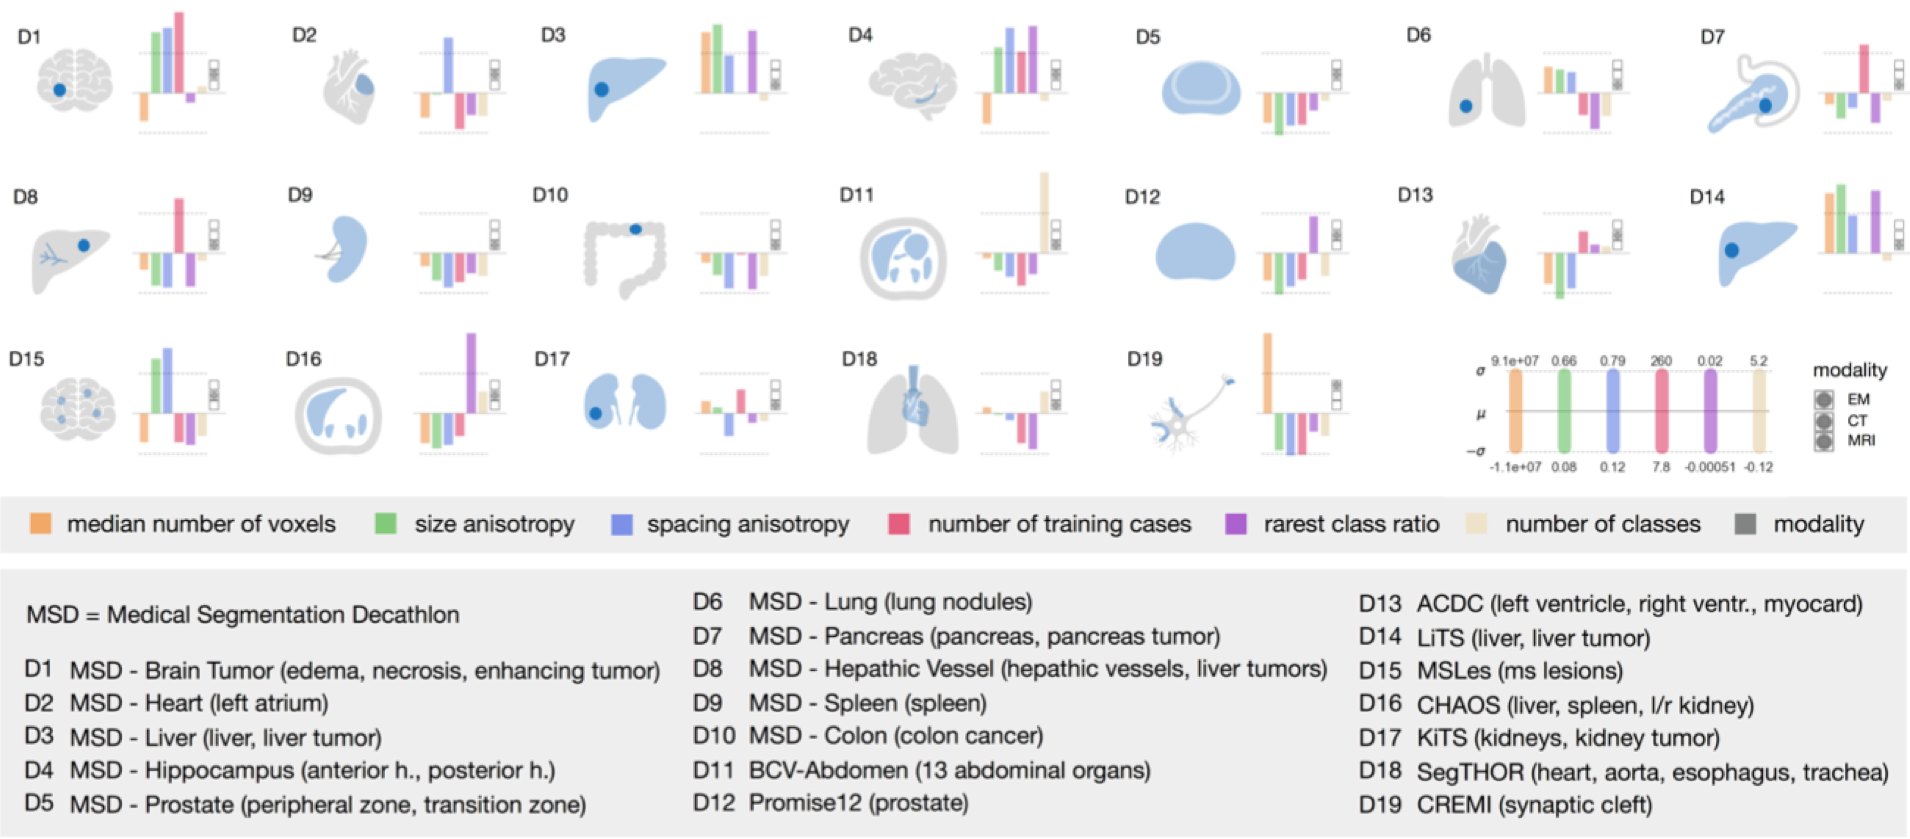
\includegraphics[scale=0.45]{Pictures/nnUnet/Bild03.png}
	\caption{Datafingerprint \cite{nnunetPaperB}}
	\label{pic:nnUnet_Datafingerprint}
\end{figure}


Aus dem Datafingerprint werden, mit Hilfe von heuristischen Regeln, die Inferred Parametern berechnet. Die Inferred Parameter umfassen die Patch Size, die Batch size, wichtige Parameter zur dynamischen Anpassung der Netzwerktopologie, wie zum Beispiel die Anzahl der Max. Poolings und Downsamplings, sowie Parameter zur Bild Vorverarbeitung. \\
Die Bestimmung der Patch size erfolgt zunächst initial über den Median der Bildgröße nach dem Resampling. Anschließend wird mit dieser Patch Size die Architektur konfiguriert und geschaut ob ausreichend GPU-Memory zur Verfügung steht. Steht nicht ausreichend GPU-Memory zur Verfügung, so wird die Patch Size reduziert und die Architektur darauf aufbauend neu konfiguriert. Dies wird so oft wiederholt, bis ausreichend GPU-Memory verfügbar ist. Anschließend wird die Batch Size angepasst und das Netzwerk abschließend konfiguriert (Siehe Abbildung \ref{pic:nnUnet_PatchSize}). Dabei muss beachtet werden, dass die Patch Size immer durch $2^i$ teilbar sein muss (mit i = Anzahl an Downsampling Operationen) da sich die Patch Size pro Downsampling Operation halbiert. Ist das nicht gegeben, so wird die Patch-Size entsprechend vergrößert oder verkleinert bis sie in allen Dimensionen durch $2^i$ teilbar ist.
 
 \begin{figure}[H]
 	
 	\centering
 	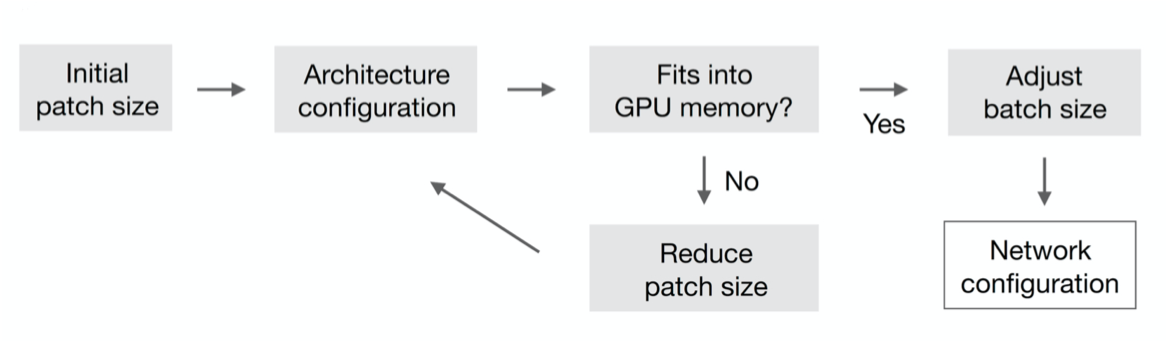
\includegraphics[scale=0.6]{Pictures/nnUnet/Bild04.png}
 	\caption{Patch Size Ermittlung \cite{nnunetPaperB} }
 	\label{pic:nnUnet_PatchSize}
 \end{figure}
 

Im Anschluss an die Inferred Parameter wird der Pipelinefingerprint erstellt, welcher sich aus den Inferred Parametern, den Blueprint Parametern und den empirischen Parametern zusammensetzt. Während die bereits beschriebenen Inferred Parameter für die entscheidende Anpassung an einen neuen Datensatz sorgen, sind die Blueprint Parameter unabhängig von dem Datensatz. Sie enthalten die drei möglichen Architekturen, sowie Hyperparameter mit festen default Werten, wie Verlustfunktion, Training Schedule, Data Augmentation, Normalisierung, stochastic Gradient oder  Aktivierungsfunktion (siehe Abbildung \ref{pic:nnUnet_Pipelinefingerprint}). Die Verlustfunktion wird als die Summe von Dice-Verlustfunktion und Cross-Entropy-Verlustfunktion gewählt. Dies wird gemacht, da medizinische Bilddaten oft Probleme mit einer großen Disbalance im Vorkommen der einzelnen Klassen haben und darum im Training seltener vorkommende Klassen unterepräsentiert sind und gleichzeitig durch die Lösung dieses Problems die Verteilung der Klassen verzerrt wird. An der Zusammensetzung dieser beiden Verlustfunktionen könnte man also auch arbeiten, wenn man das Framework auf andere Arten von Datensätzen anpassen wollte. Das Training läuft über 1000 Epochen mit jeweils 250 Trainingsiterationen. 

\begin{figure}[H]
	
	\centering
	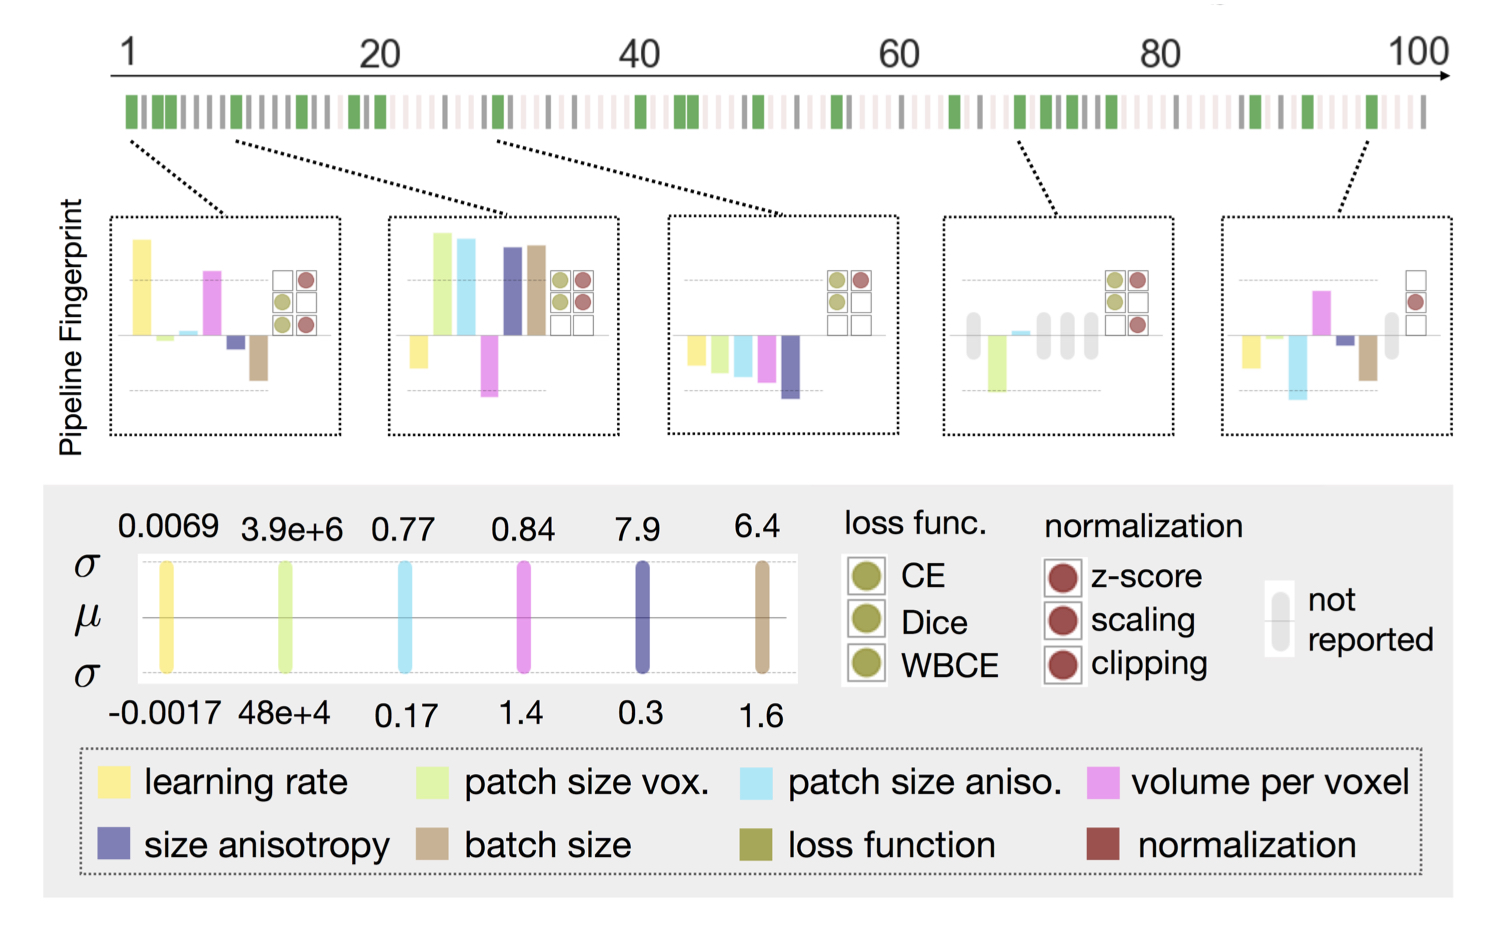
\includegraphics[scale=0.5]{Pictures/nnUnet/Bild05.png}
	\caption{Pipelinefingerprint \cite{nnunetPaperB} }
	\label{pic:nnUnet_Pipelinefingerprint}
\end{figure}

Da die empirischen Parameter nicht direkt aus dem Datensatz erschlossen werden können, werden sich nach dem Training empirisch bestimmt. Sie werden zur Nachbearbeitung und bei der Auswahl der besten Netzstruktur genutzt. 


\section{Unsere Arbeit / Praxis}
\todo{Durchschnitt ermitteln Pascal VOC 2012}
\todo{Predictions fuer Task 100 CT alle Versionen auswerten}
\begin{figure}[H]
\begin{tabular}{|c|c|c|c|c|c|}
\hline 
\multirow{3}{*}{Datensatz} &  &  & & Train-& Test- \\ 
 & Split & verwendete & Trainingszeit & Accuracy& Accuracy \\ 
 & (Train:Test) & nnUNet-Variante & (h) & (Dice)& (Dice)  \\ 
\hline 
Larven & 265:0 $\approx$ 1:0 & 2D & 8:30 & 0.99970 & - \\ 
\hline 
Larven & 173:92 $\approx$ 2:1 & 2D & 6:45 & 0.99982 & 0.94459 \\ 
\hline 
Pascal VOC12 & 2516:340 $\approx$ 7:1 & 2D & 26:00 & 0.90266 & 0.34953 \\ 
\hline 
Retina-2D (manuelle & \multirow{2}{*}{56:34 $\approx$ 2:1} & \multirow{2}{*}{2D} & \multirow{2}{*}{23:20} & \multirow{2}{*}{0.99977} &\multirow{2}{*}{0.93606}  \\ 
Data-Augmentation)&  & & & &  \\ 
\hline 
Retina-2D (minimal) & 13:32 $\approx$ 1:2 & 2D & 21:15 & 0.99999 &  0.83013 \\ 
\hline 
CT & 19:0 $\approx$ 1:0 & 3D\_fullres & 58:30  & ? & - \\ 

\hline 
\multirow{2}{*}{CT} & \multirow{2}{*}{19:0 $\approx$ 1:0} & \multirow{2}{*}{3D\_fullres} & $\approx$ 89:30  & \multirow{2}{*}{?} & \multirow{2}{*}{-} \\ 
 &  &  & (\textbf{2000} Epochen) &  &  \\ 
\hline 
CT & 19:0 $\approx$ 1:0 & 2D & 19:00 & ? & - \\ 
\hline 
\multirow{2}{*}{CT} & \multirow{2}{*}{19:0 $\approx$ 1:0} & \multirow{2}{*}{3D\_cascade} & $\approx$ 53:00 + 49:30 & \multirow{2}{*}{?} & \multirow{2}{*}{-} \\ 
 &  &  & =102:30 &  & \\ 
\hline 
Retina-3D & 14:7 $\approx$ 2:1 & 3D\_fullres & 45:15 & 0.91863 & 0.83759 \\ 
\hline 
Retina-3D & 14:7 $\approx$ 2:1  & 2D & 19:00 & 0.98574 & 0.78931 \\ 
\hline 
Retina-3D (Ensemble) & 14:7 $\approx$ 2:1 & 2D \& 3D\_fullres & - & 0.97775 & 0.82363 \\ 
\hline
\end{tabular} 
\caption{Datensätze, auf denen wir trainiert haben (jeweils 1000 Epochen auf GPUv100)}
\label{tab:Training}
\end{figure}

Grundsätzlich haben wir für jeden folgenden Datensatz die Ursprungsdateien in Nifti-Dateien umgewandelt und meistens zufällig in einen Train- und Testsplit aufgeteilt, außer bei dem 3D-CT Datensatz, da wird dort auch mit allen Samples im Trainsplit keine sonderlich guten Ergebnisse erzielen konnten, und dem ersten Versuch auf dem Larvendatensatz.\\
Der generelle Arbeitsablauf bestand bei uns aus der Befehlsabfolge:
\begin{lstlisting}[language=bash]
nnUNet_plan_and_preprocess -t <TASK-ID> --verify_dataset_integrity
\end{lstlisting}
bzw. für 2D-Datensätze, da dort kein 3D-Modell anwendbar ist:
\begin{lstlisting}[language=bash]
nnUNet_plan_and_preprocess -t <TASK-ID> -pl3d None
\end{lstlisting}
Dieser Befehl bereitet das Training vor und prüft, ob der gegebene Datensatz als Nifti-Dateien korrekt ist, indem Wertebereiche und das Vorhandensein aller Dateien geprüft wird. Da dieser Befehl das Training vorbereitet, muss er mit den gleichen verfügbaren Ressourcen wie auch später das Training aufgerufen werden, in unserem Fall auf dem GPUv100 Knoten von Palma II.\\\\
Danach kann das Training für die einzelnen Netzvarianten (2d, 3d\_fullres, 3d\_cascade gestartet werden:
\begin{lstlisting}[language=bash]
# 2d
nnUNet_train 2d nnUNetTrainerV2 <TASK-ID> all --npz
# 3d_fullres
nnUNet_train 3d_fullres nnUNetTrainerV2 <TASK-ID> all --npz
# Cascade
nnUNet_train 3d_lowres nnUNetTrainerV2 <TASK-ID> all --npz
nnUNet_train 3d_cascade_fullres nnUNetTrainerV2CascadeFullRes
	 <TASK-ID> all --npz
\end{lstlisting}
Dabei verwenden wir für 3D-Datensätze immer 3d\_fullres und die 2d-Variante, für 2D-Datensätze immer nur die 2d Variante. Falls das Framework es für einen 3D-Datensatz notwendig hält bzw. überhaupt zulässt, wird auch 3d\_cascade verwendet.
Der Parameter --npz sorgt dafür, dass die Softmax-Ausgaben zusätzlich gespeichert werden, was zwar sehr viel Festplattenspeicher benötigt, uns aber später ein eventuelles Ensembling der Predictions ermöglicht.\\
Der Parameter \enquote{all} gibt an, welcher der 5 Folds, die das Framework automatisch erstellt, zur Validierung benutzt wird, während die anderen 4 dem Training dienen.
Der Autor des Frameworks vermutet, dass wenn man statt \enquote{all} alle Werte 0 bis 4 verwendet und hinterher aus den 5 verschiedenen Folds ein Ensemble bildet die finale Performance besser ist im Vergleich zu \enquote{all}, jedoch hat auch er keine empirischen Beweise dafür \cite{nnunetGithub-Folds}. Wir haben uns für \enquote{all} entschieden, da die Handhabung dann etwas einfacher wird und wir vermuten, dass die zum Training benötigte Zeit deutlich geringer ist, da lediglich ein Modell aus allen Trainingsdaten trainiert wird, und nicht 5 verschiedene basierend auf einer verschiedener Aufteilung der Folds. Außerdem sind unsere Ergebnisse trotz der nicht optimalen Wahl der Parameter ziemlich gut (s. Tabelle \ref{tab:Training}). \\
Nach dem Beenden des Trainings lassen wir uns von dem Framework die Predictions zu dem Train- und Testsplit erzeugen:
\begin{lstlisting}[language=bash]
nnUNet_predict -i <Pfad zu Original-Niftis> -o <Prediction-Pfad>
 -m <2d, 3d_fullres oder 3d_cascade_fullres> -t <TASK-ID> -f all -z
\end{lstlisting}
Der Parameter -z sorgt auch hier wieder für das Speichern der Softmax-Werte, um später eventuell ein Ensembling aus verschiedenen Netzvarianten zu bilden.\\\\
Abschließend erstellen wir mit dem Framework eine Auswertung der Performance auf dem Datensatz, indem wir für den Train- und Testsplit die Ground-Truth Segmentierung mit den Predictions vergleichen:
\begin{lstlisting}[language=bash]
nnUNet_evaluate_folder -ref <Ground-Truth-Pfad>
 -pred <Prediction-Pfad> -l <Klassennummern>
\end{lstlisting}
<Klassennummern> ist hierbei eine Liste aller Klassennummern, die in der Auswertung berücksichtigt werden. Da uns die Performance auf dem Hintergrund (0) nicht interessiert, starten wir bei 1 und gehen z.B. bei Pascal VOC12 \cite{PascalVOCDatensatz} alle Klassen durch \textit{-l 1 2 3 4 ... 20}. Die erzeugt in dem Ordner, in dem die Predictions liegen eine JSON-Datei mit ausführlichen Informationen über die Güte der Predictions je Sample und je vorhandener Klasse, aus der wir einen Scatterplot erstellen.



% Aufteilung in 2D/3D erstmal weggemacht, ich gehe chronologisch durch

\subsection{Datensätze aus dem Paper}
Nach unseren schlechten vorherigen Erfahrungen mit (Auto-) Deeplab \cite{deeplabGithub} und insbesondere NAS-Unet \cite{nasunetGithub} haben wir zuerst versucht die bemerkenswert guten Ergebnisse \parencite[Kapitel 4, Table 2]{nnunetPaper} auf den Datensätzen der Medical Segmentation Decathlon Challenge \cite{msdChallenge} mit dem Framework zu reproduzieren. Wir haben die 3D-Datensätze Spleen, Lung und Heart \cite{msdChallenge} ausprobiert und konnten auf allen ähnliche Ergebnisse wie im Paper erzielen.\\

\subsection{Larven-Datensatz}
\subsubsection{Larven-Datensatz ohne Testsplit}
\begin{figure}[H]
\centering
\includesvg[height=6.5cm]{Pictures/nnUnet/Praxis/Task200-Larven-nur-train/Haeufigkeitsverteilung-200-Larven-Train}
\caption{Anteil von Objekt (Larve) je Sample im Trainsplit (alle 265 Samples) mit Durchschnitt $\approx$ 5,8\%}
\label{pic:Haeuf_200}
\end{figure}
Nachdem wir die Ergebnisse im Paper erfolgreich reproduzieren konnten haben wir versucht einen eigenen Datensatz in das Framework zu geben. Dabei ist zu erwähnen, dass unser Larven-Datensatz ein 2D Datensatz ist. Er beinhaltet Graustufen-Bilder von Larven auf einer Glasscheibe, die mittels Frustrated Total Internal Reflection abgelichtet wurden. Ziel ist es, die Larven zu segmentieren und die Verschmutzungen um die Larven herum dabei zu ignorieren. Jedoch ist nnUNet nicht dafür entworfen worden auf 2D-Datensätze angewendet zu werden, besonders wenn die Datensätze aus der \enquote{non-biomedical domain} \cite{nnunetGithub2D-Daten} stammen.\\
Dies ist jedoch nicht als Einschränkung des Funktionsumfangs zu verstehen, sondern lediglich als Vorwarnung, dass die Ergebnisse eventuell nicht gut ausfallen werden.\\\\
Wir haben das zum Framework gehörige Python-Script \cite{nnunetGithub2D-Pythonscript} nur leicht modifizieren müssen und konnten den 2D Datensatz in Nifti-Dateien (.nii.gz) konvertieren und so in das Framework geben.\\
Da es sich hierbei um unseren ersten Test des Frameworks mit eigenem Datensatz handelte haben wir zuerst keinen Test-Split vorgesehen und alle 265 Bilder als Trainingsdaten benutzt.
\begin{figure}[H]
\centering
\begin{minipage}{.6\textwidth}
\begin{subfigure}{\textwidth}
\centering
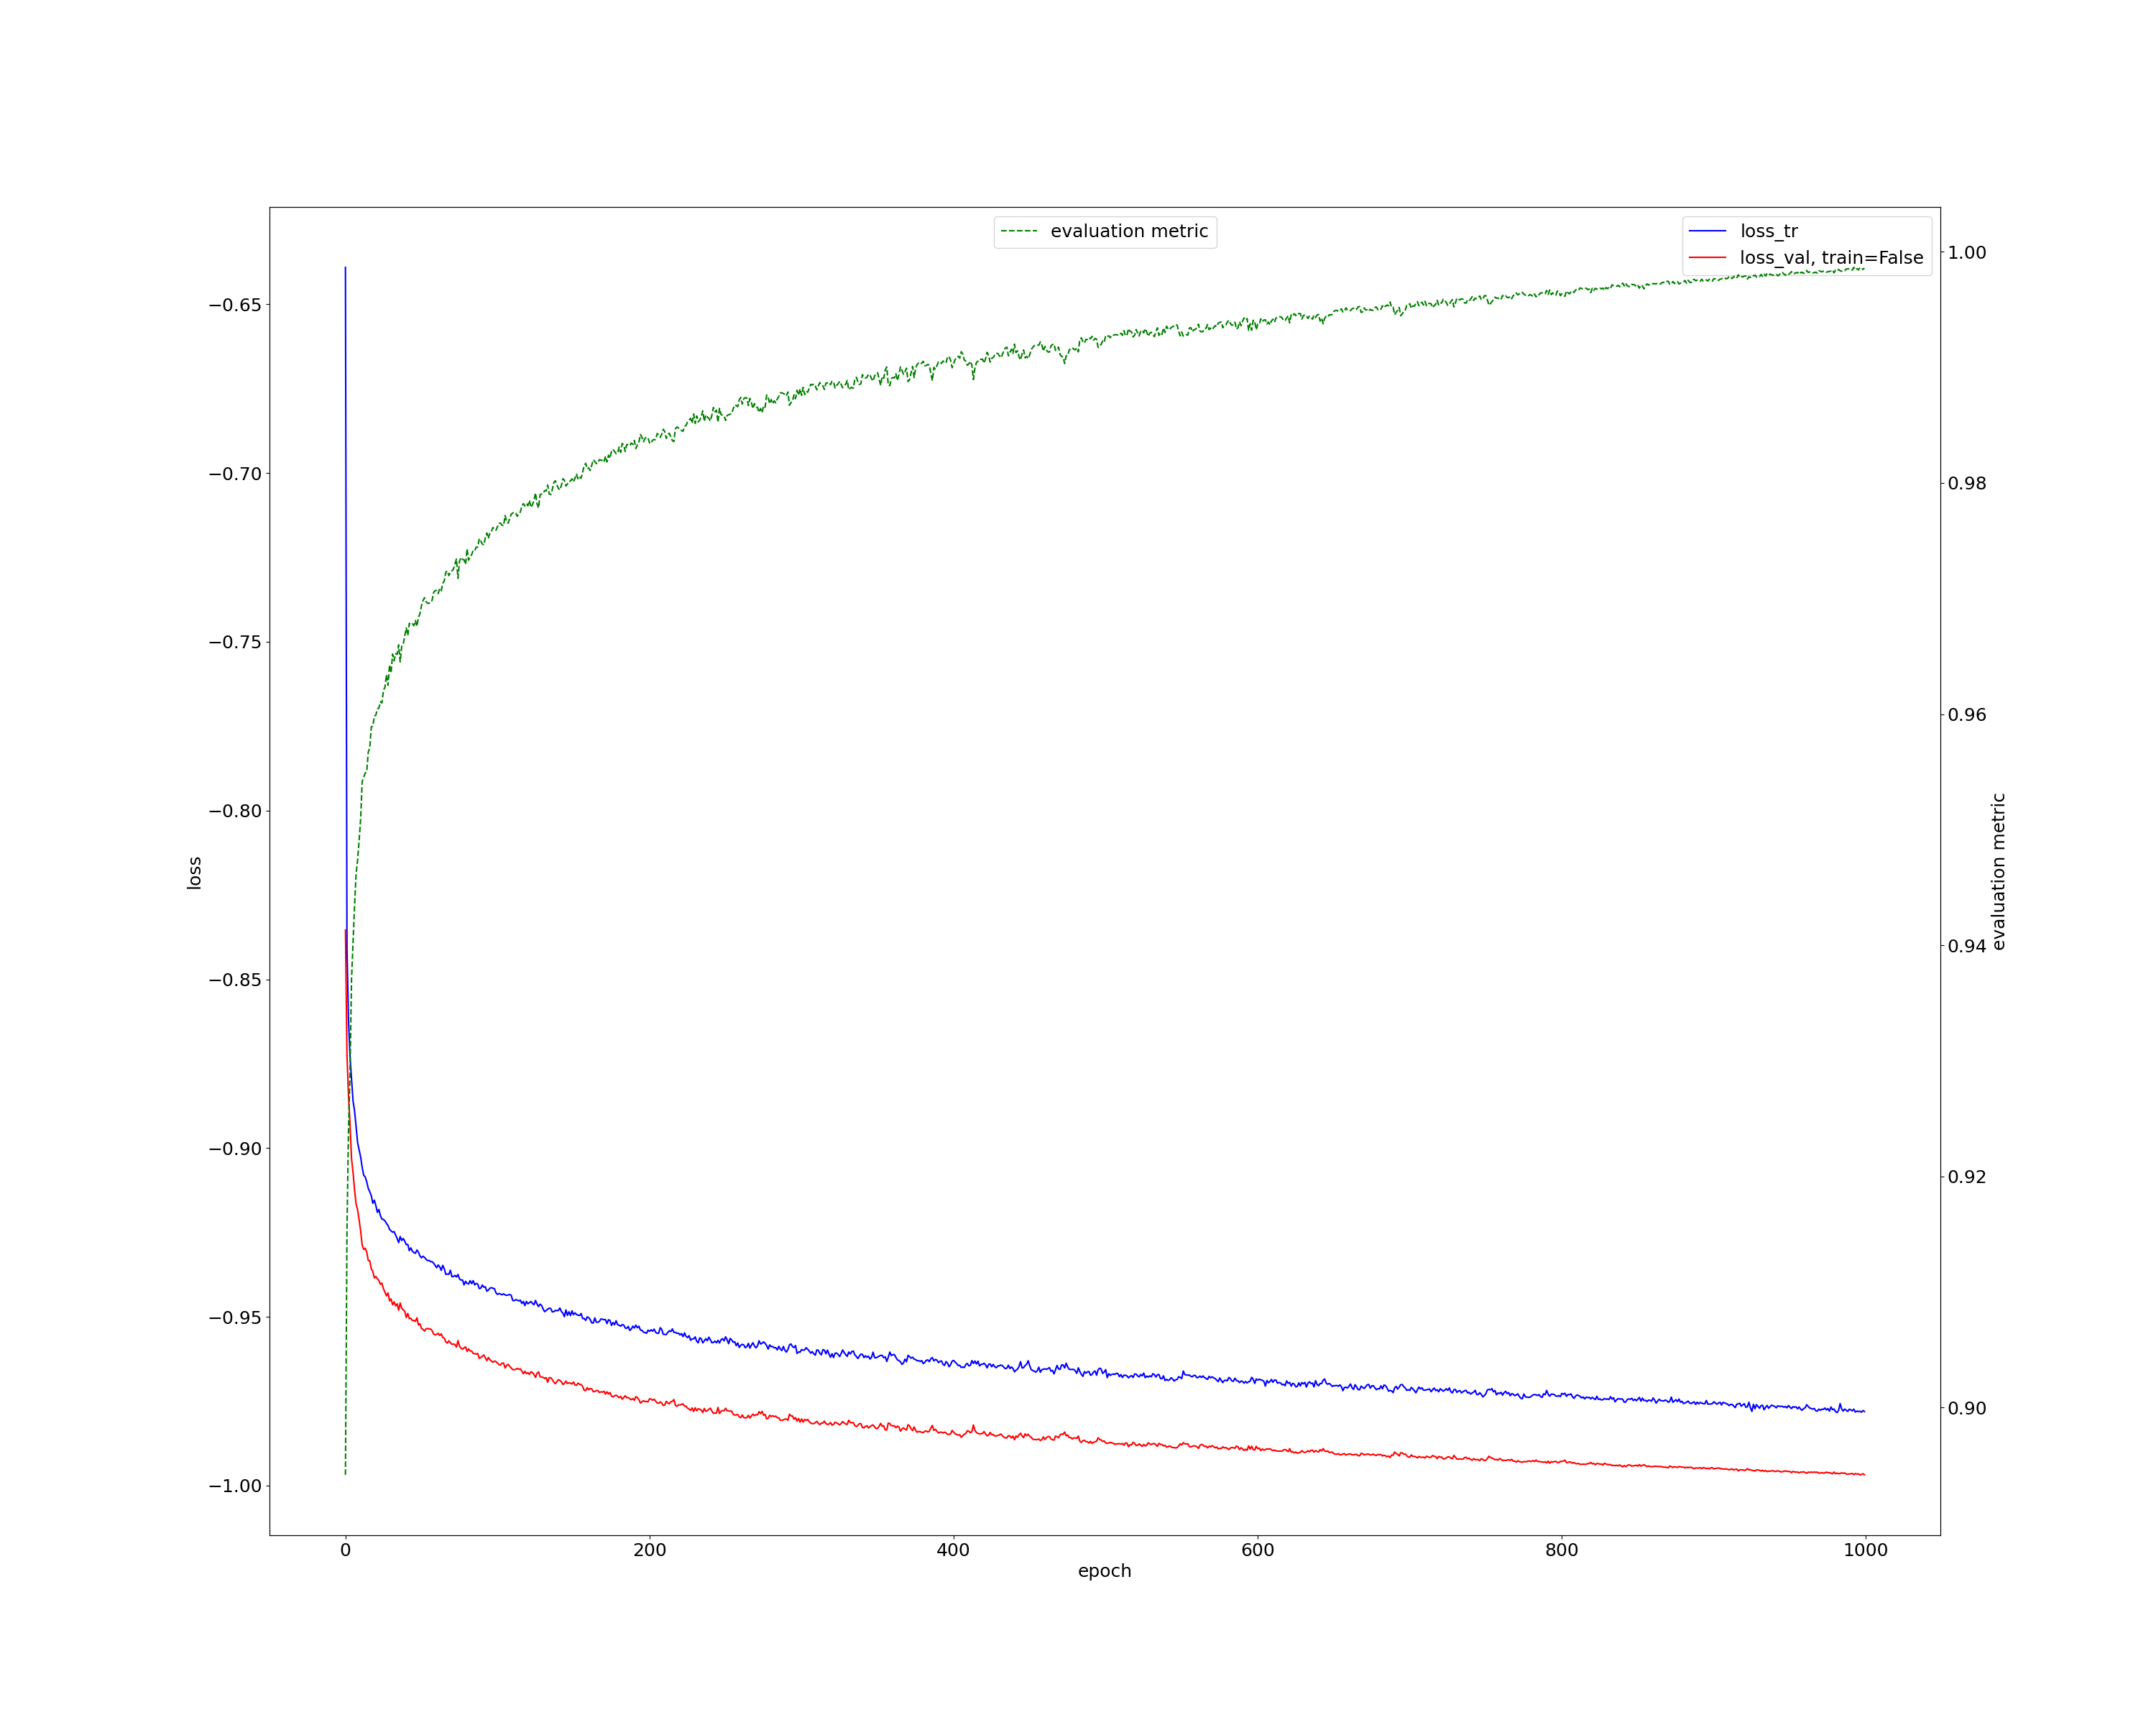
\includegraphics[width=\textwidth]{Pictures/nnUnet/Praxis/Task200-Larven-nur-train/progress_200-Larven-nur-train.png}
\caption{Verlauf des Dice-Koeffizienten beim Training über 1000 Epochen}
\label{pic:Prog_200}
\end{subfigure}
\end{minipage}%
\begin{minipage}{.4\textwidth}
\begin{subfigure}{\textwidth}
\includesvg[width=\textwidth]{Pictures/nnUnet/Praxis/Task200-Larven-nur-train/Scatterplot-Dice-200-Larven-Train}
\caption{Scatterplot der Dice-Koeffizienten je Sample (265 Stück)}
\label{pic:Dice_200}

\end{subfigure}
\end{minipage}
\caption{Dice-Koeffizienten auf dem Trainsplit zum Larvendatensatz ohne Testsplit}
\end{figure}

\begin{figure}[H]
\centering
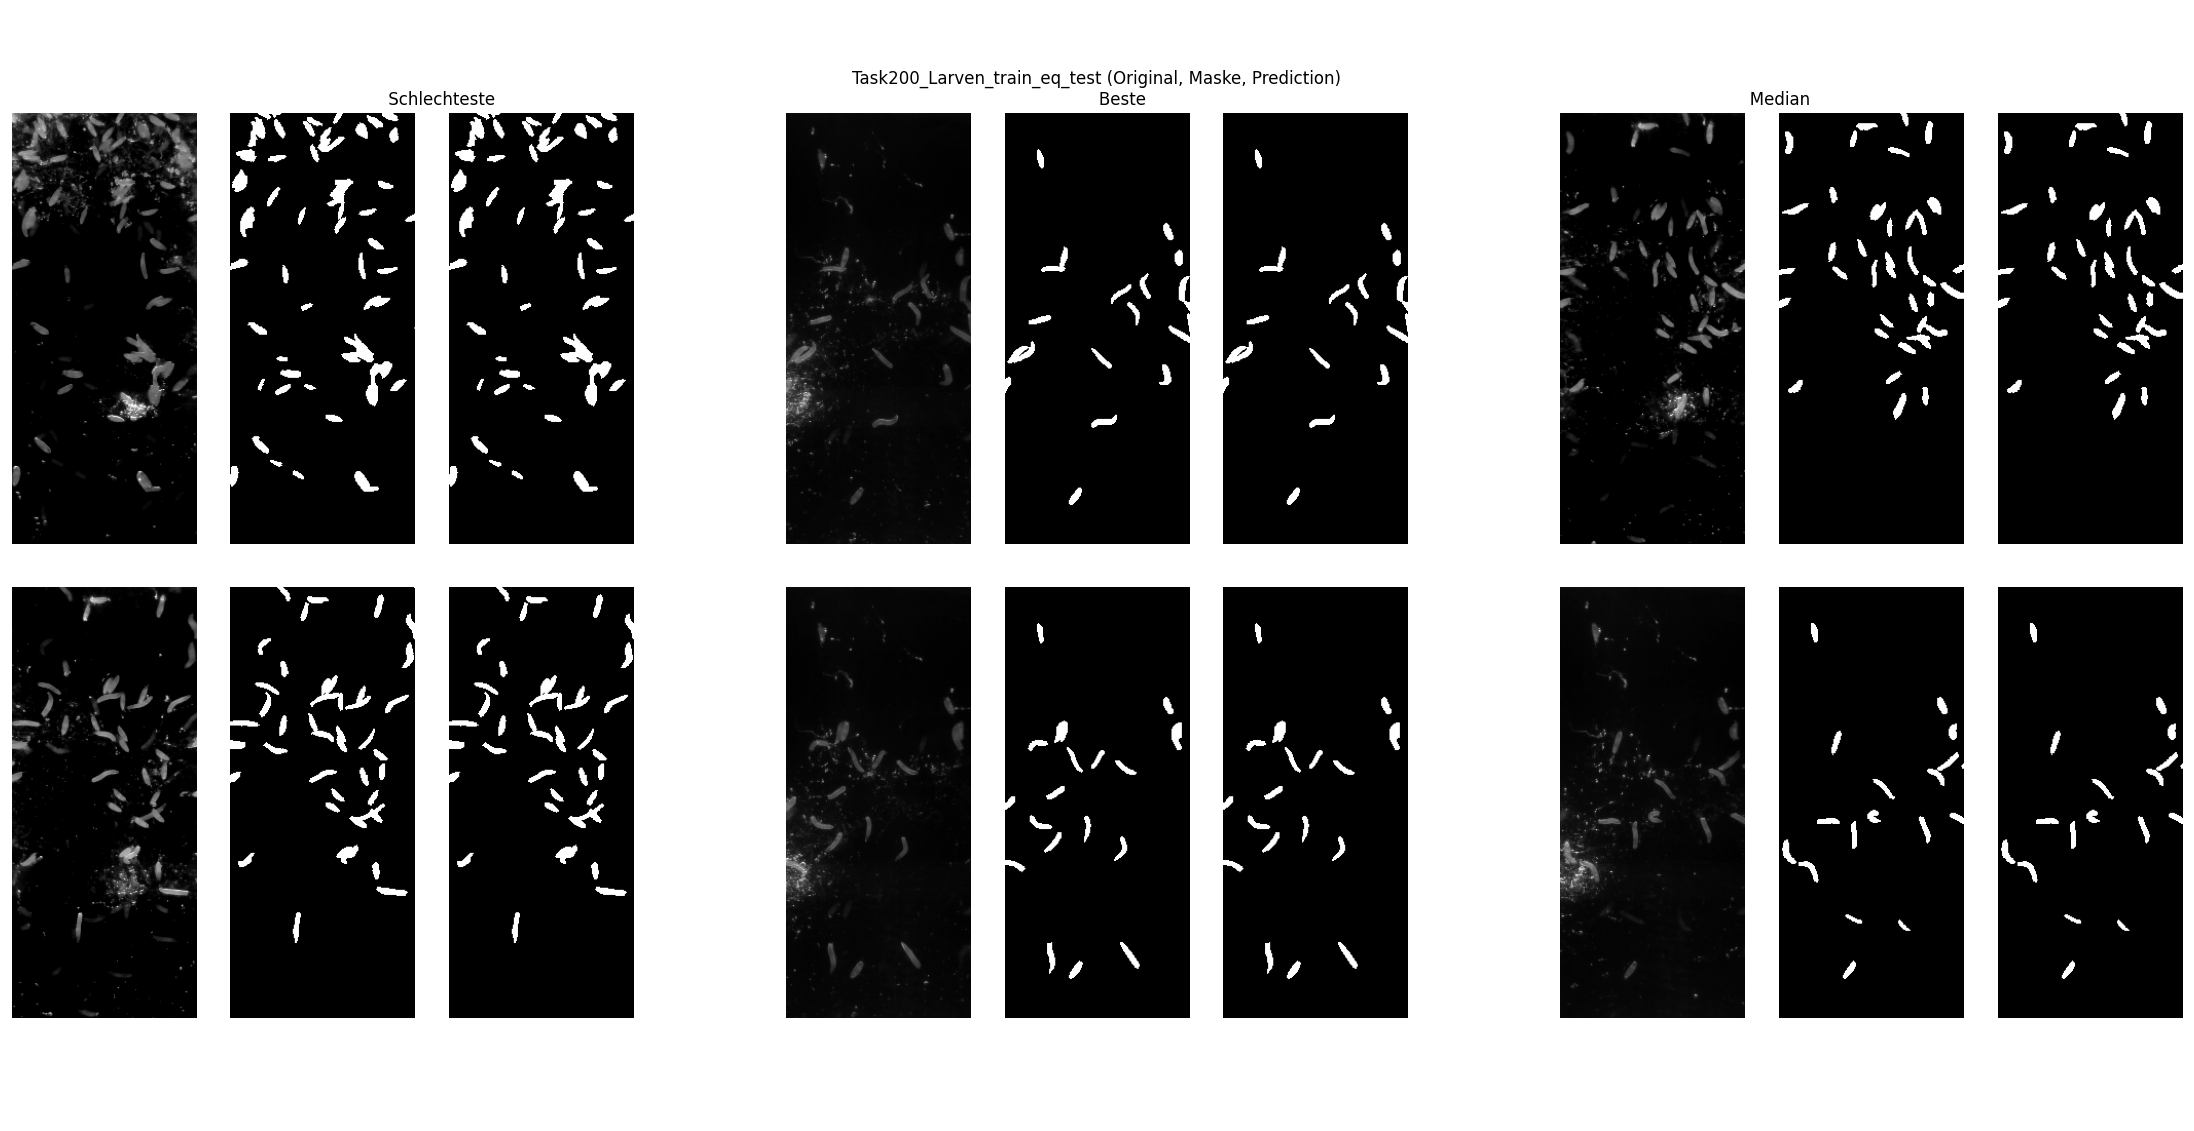
\includegraphics[height=0.35\textheight, width=\textwidth]{Pictures/nnUnet/Praxis/Task200-Larven-nur-train/Vis-Train.png}
\caption{Visualisierung des Trainsplits auf dem Larvendatensatz ohne Testsplit (links: schlechteste Ergebnisse, mitte: beste Ergebnisse, rechts: Ergebnisse im Median; jeweils Original, Ground-Truth und Prediction)}
\label{pic:Vis-Train_200}

\end{figure}
Wir konnten bei unserem ersten Versuch einen eigenen Datensatz in das Framework zu geben einen Dice-Wert von durchschnittlich $> 0.999$ erzielen und auch die am schlechtesten segmentierten Samples liegen weit über $0.99$, wie in Abbildung \ref{pic:Dice_200} zu erkennen ist.
Auch bei der Visualisierung der besten, schlechtesten und mittleren Ergebnisse (Abbildung \ref{pic:Vis-Train_200}) kann man zwischen Ground-Truth und der Prediction mit bloßem Auge keine Unterschiede erkennen.
\subsubsection{Larven-Datensatz mit $\frac{2}{3}$ Train- und $\frac{1}{3}$ Testsplit}
Anschließend haben wir die Larvenbilder zufällig in $\frac{2}{3}$ Trainingsdaten und $\frac{1}{3}$ Testdaten aufgeteilt und erneut trainieren lassen. Wir haben uns vergewissert, dass Train- und Testsplit möglichst allgemein und zueinander ähnlich sind, und nicht zufällig in einem Split nur die Samples mit hohem Objektanteil und im anderen mit wenig Objektanteil vorhanden sind. Sowohl im Train- als auch im Testsplit ist der Objektanteil in den Samples ähnlich (s. Abbildung \ref{pic:Haeuf_201}).
\begin{figure}[H]
\begin{minipage}{.5\textwidth}
\begin{subfigure}{\textwidth}
\includesvg[width=\textwidth]{Pictures/nnUnet/Praxis/Task201-Larven-drittel-testsplit/Haeufigkeitsverteilung-201-Larven-Train}
\caption{Trainsplit}
\label{pic:Haeuf-Train_201}
\end{subfigure}
\end{minipage}
\begin{minipage}{.5\textwidth}
\begin{subfigure}{\textwidth}
\includesvg[width=\textwidth]{Pictures/nnUnet/Praxis/Task201-Larven-drittel-testsplit/Haeufigkeitsverteilung-201-Larven-Test}
\caption{Testsplit}
\label{pic:Haeuf-Test_201}
\end{subfigure}
\end{minipage}
\caption{Anteil von Objekt (Larve) je Sample mit Durchschnitt je Split $\approx$ 5,8\%}
\label{pic:Haeuf_201}
\end{figure}

Hierbei konnten wir nach dem Training mit Hilfe des Testsplits die Performance des erlernten Modells evaluieren und prüfen, ob das Framework tatsächlich gelernt hat die Strukturen und Merkmale einer Larve zu erkennen und von ähnlich aussehender Verschmutzung zu unterscheiden. Auf dem Testsplit ist die Performance etwas schlechter als auf dem Trainsplit, aber mit einem Dice-Koeffizienten von über $0.94$ im Durchschnitt trotzdem noch erstaunlich gut und selbst das am schlechtesten segmentierte Sample im Testsplit hat mit $0.9$ auch noch eine akzeptable Genauigkeit (s. Abbildung \ref{pic:Dice_201}).

\begin{figure}[H]
\centering
\begin{minipage}{.6\textwidth}
\begin{subfigure}{\textwidth}
\centering
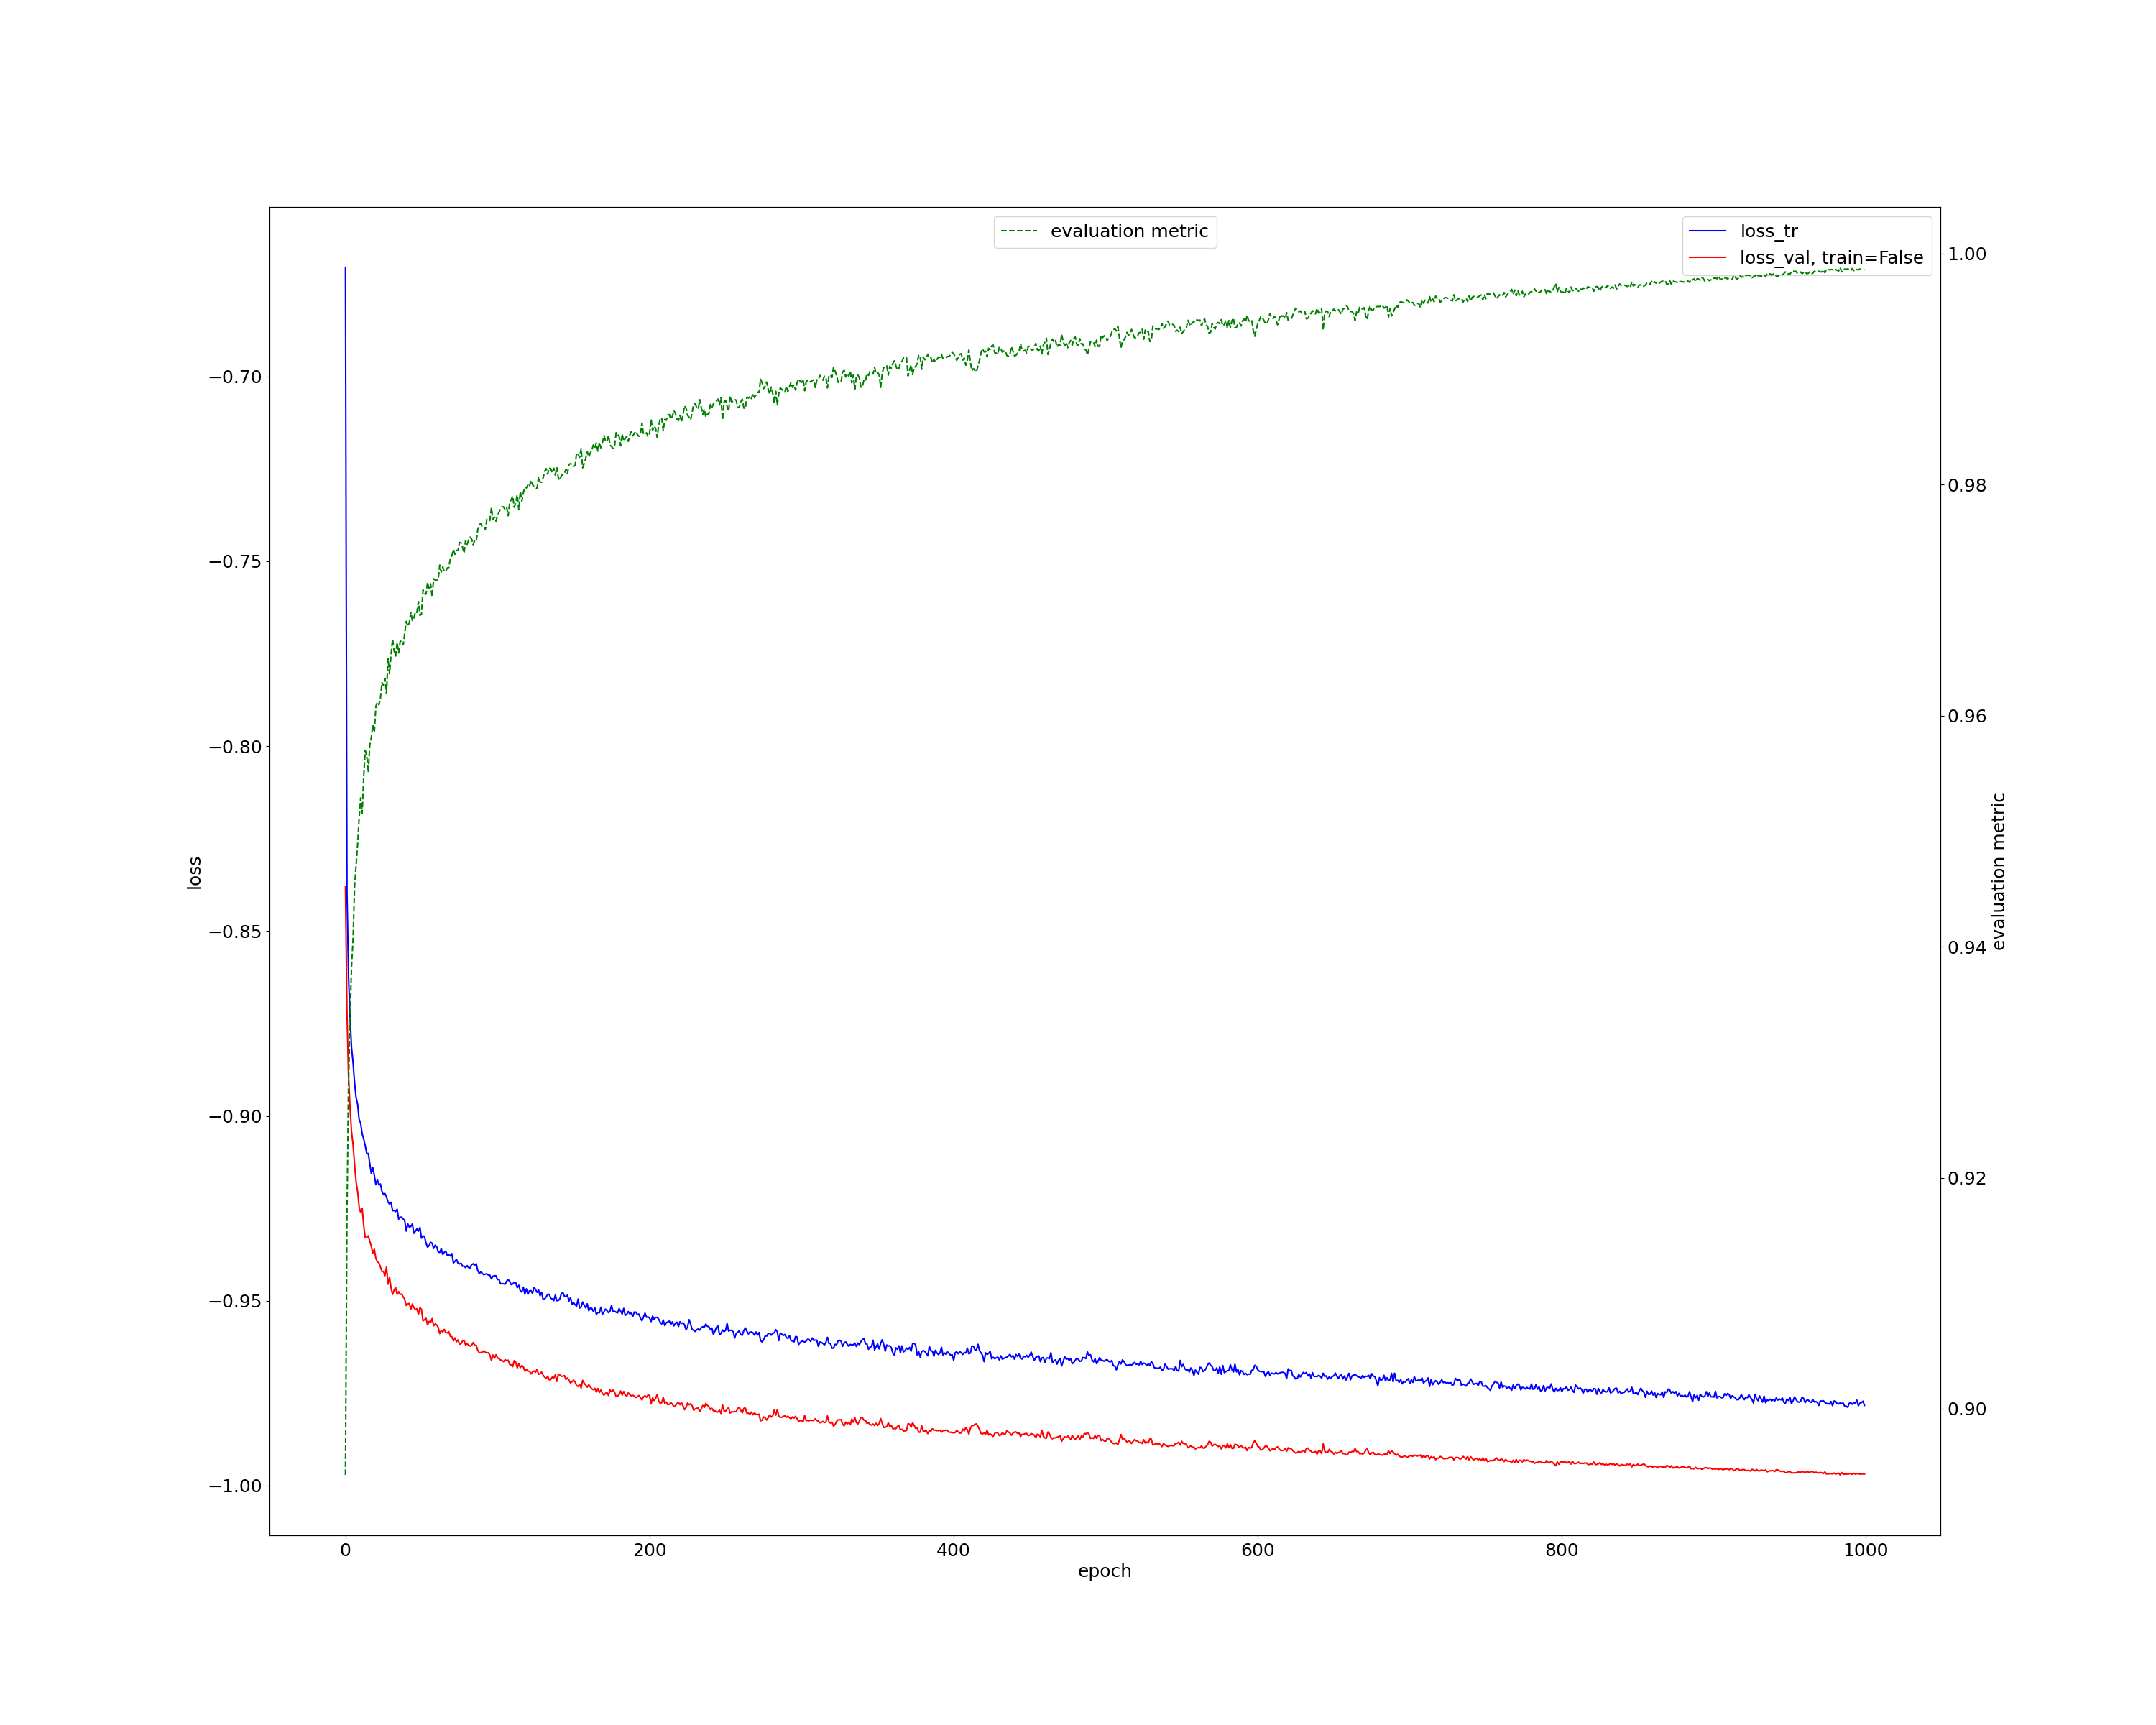
\includegraphics[width=\textwidth]{Pictures/nnUnet/Praxis/Task201-Larven-drittel-testsplit/progress_201-Larven-drittel-testsplit.png}
\caption{Verlauf des Dice-Koeffizienten beim Training über 1000 Epochen}
\label{pic:Prog_201}
\end{subfigure}
\end{minipage}%
\begin{minipage}{.4\textwidth}
\begin{subfigure}{\textwidth}
\includesvg[width=\textwidth]{Pictures/nnUnet/Praxis/Task201-Larven-drittel-testsplit/Scatterplot-Dice-201-Larven}
\caption{Scatterplot der Dice-Koeffizienten je Sample für Train- und Testsplit}
\label{pic:Dice_201}
\end{subfigure}
\end{minipage}

\caption{Dice-Koeffizienten zum Larvendatensatz mit einem Drittel als Testsplit}
\end{figure}

Bei der Visualisierung der Predictions fällt erneut auf, dass auf dem Trainsplit mit bloßem Auge keine Unterschiede zu Ground-Truth vorhanden sind (s. Abbildung \ref{pic:Vis-Train_201}), bei dem Testsplit kommt es jedoch bei den schlechtesten Beispielen zu Fehlern, die auch deutlich erkennbar sind. Es werden teilweise komplette Larven nicht oder nur teilweise erkannt und zudem wird auch besonders in den stark verschmutzen Bildern die Verschmutzung als Larve erkannt. Hierbei stellt sich die Frage, ob die Ground-Truth Segmentierung korrekt ist, da besonders die angeblichen Verschmutzungen, die das Modell als Larve erkannt hat, im Originalbild tatsächlich eher wie eine Larve aussehen als Verschmutzung. Intuitiv würde man die betroffenen Stellen im Originalbild vermutlich auch, wie das Modell, als Larve interpretieren. Die Larven die nicht erkannt wurden sind sehr schwach bis gar nicht mit dem Auge erkennbar bzw. ähneln stark einer Verschmutzung (s. Abbildung \ref{pic:Vis-Test_201}).

\begin{figure}[H]
\centering
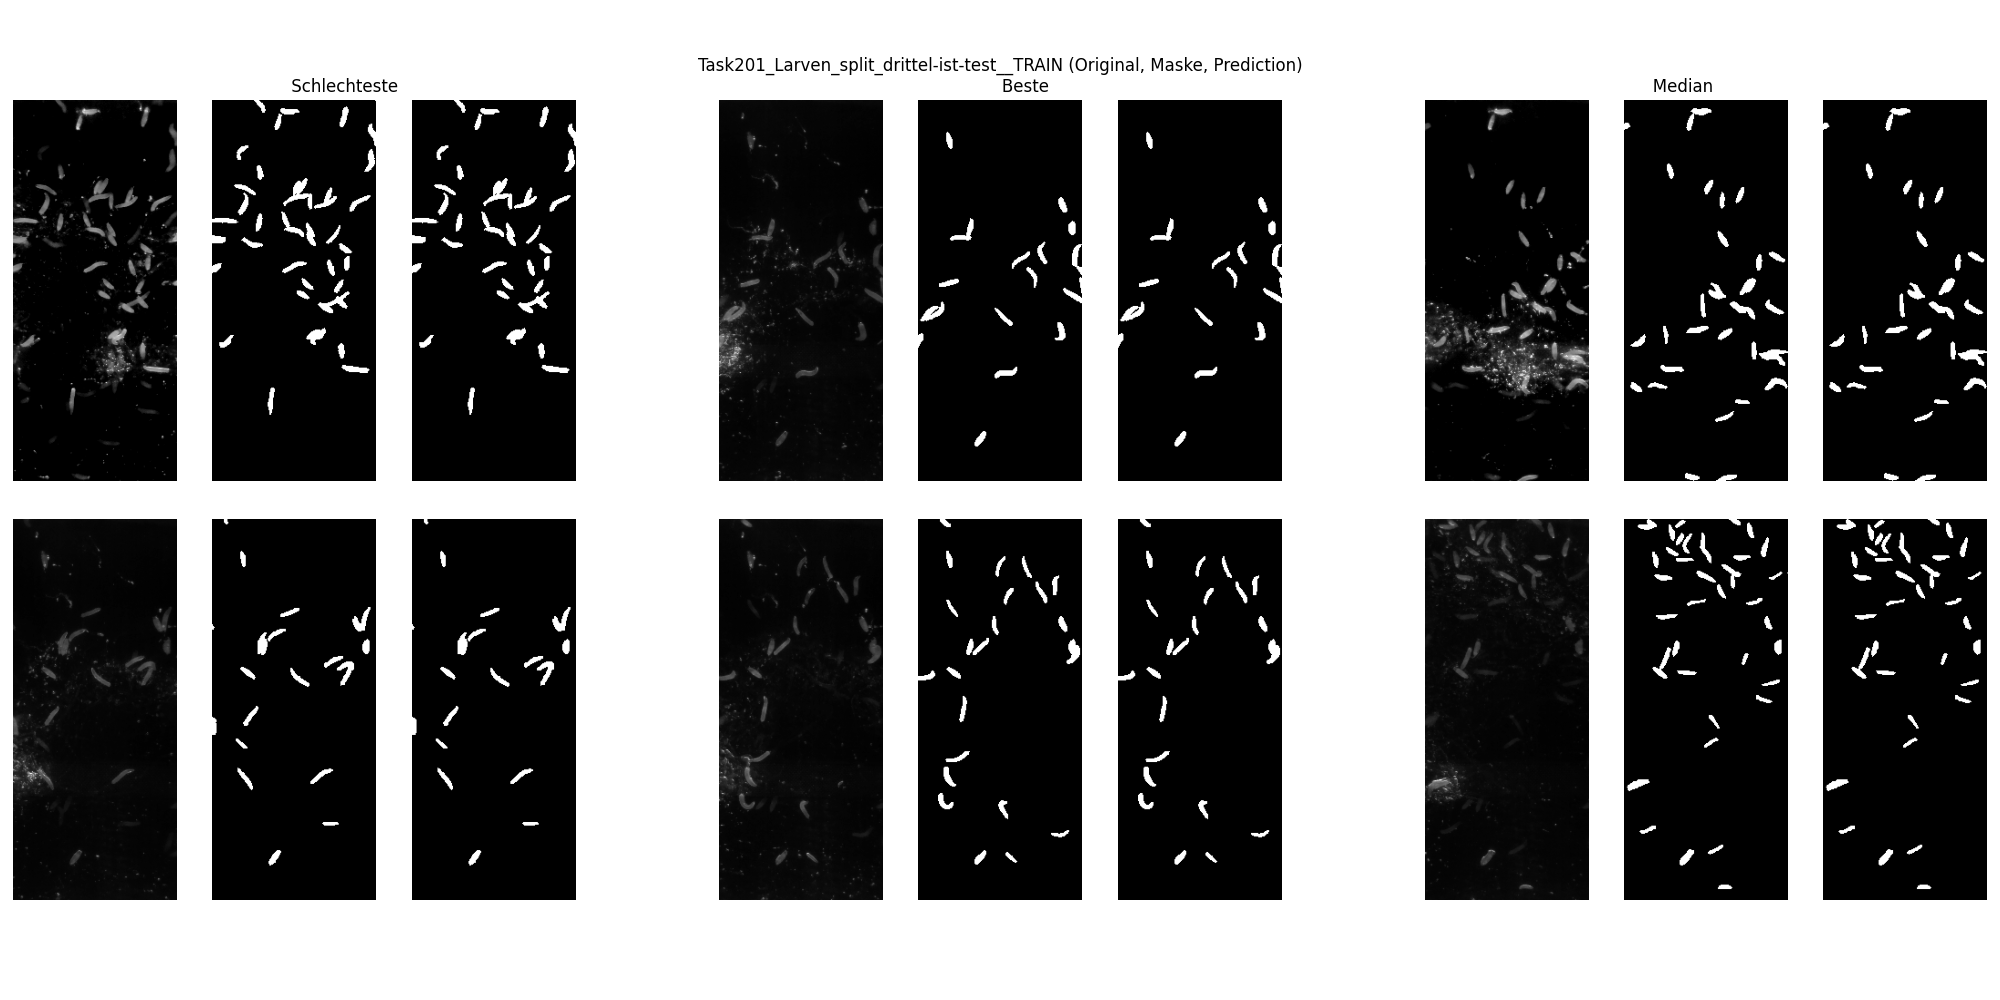
\includegraphics[height=0.35\textheight, width=\textwidth]{Pictures/nnUnet/Praxis/Task201-Larven-drittel-testsplit/Vis-Train.png}
\caption{Visualisierung des Trainsplits auf dem Larvendatensatz mit $\frac{1}{3}$ Testsplit (links: schlechteste Ergebnisse, mitte: beste Ergebnisse, rechts: Ergebnisse im Median; jeweils Original, Ground-Truth und Prediction)}
\label{pic:Vis-Train_201}
\end{figure}


\begin{figure}[H]
\centering
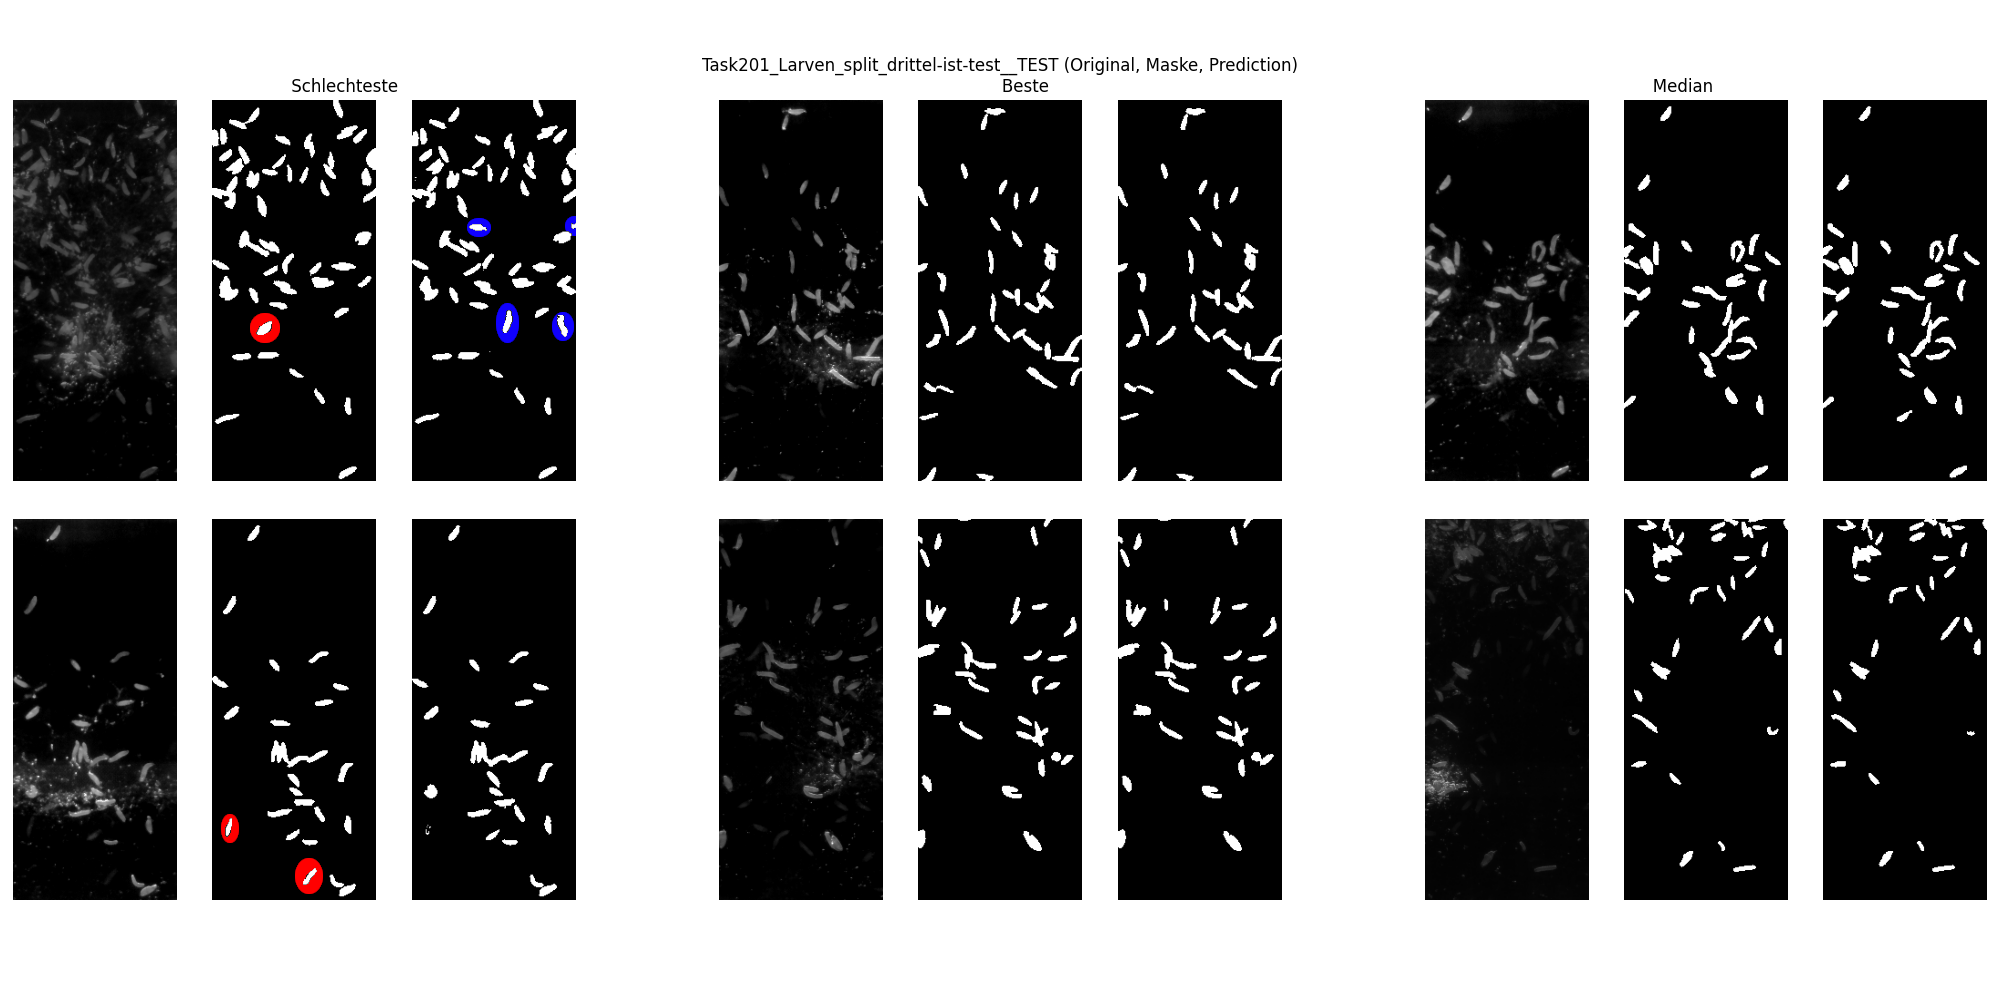
\includegraphics[height=0.35\textheight, width=\textwidth]{Pictures/nnUnet/Praxis/Task201-Larven-drittel-testsplit/Vis-Test-markiert.png}
\caption{Visualisierung des Testsplits auf dem Larvendatensatz mit $\frac{1}{3}$ Testsplit (links: schlechteste Ergebnisse, mitte: beste Ergebnisse, rechts: Ergebnisse im Median; jeweils Original, Ground-Truth und Prediction). Rot eingefärbt sind nicht erkannte Larven, blau als Larven erkannte Verschmutzungen}
\label{pic:Vis-Test_201}
\end{figure}


\subsection{Retina 2D-Datensatz}
\begin{figure}[H]
\begin{minipage}{.5\textwidth}
\begin{subfigure}{\textwidth}
\includesvg[width=\textwidth]{Pictures/nnUnet/Praxis/Task205-Augen-minimal-13-trainsamples/Haeufigkeitsverteilung-205-Retina2D-minimal-Train}
\caption{Trainsplit}
\label{pic:Haeuf-Train_205}
\end{subfigure}
\end{minipage}
\begin{minipage}{.5\textwidth}
\begin{subfigure}{\textwidth}
\includesvg[width=\textwidth]{Pictures/nnUnet/Praxis/Task205-Augen-minimal-13-trainsamples/Haeufigkeitsverteilung-205-Retina2D-minimal-Test}
\caption{Testsplit}
\label{pic:Haeuf-Test_205}
\end{subfigure}
\end{minipage}
\caption{Anteil von Objekt (Ader) je Sample mit Durchschnitt je Split $\approx$ 11-12\%}
\label{pic:Haeuf_205}
\end{figure}

Da wir auf dem Larven-Datensatz (Graustufen mit einer einzigen Objekt-Klasse) so gute Ergebnisse erzielen konnten, obwohl das Framework für solche Aufgaben eigentlich nicht gemacht ist, wollten wir einen Schritt weiter gehen und statt graustufen Bildern farbige Bilder verwenden.\\
Dazu verwenden wir den Retina-2D Datensatz \cite{retina2d}. Dieser besteht aus jeweils 15 Aufnahmen von gesunden Retinae, Retinae von Augen mit Glaukom und diabetischer Retinopathie, also insgesamt 45 hochauflösenden RGB-Bildern. Unser Ziel der Segmentierung ist es, unabhängig von der Erkrankung, die Adern in der Retina zu markieren.\\
Diese Bilder konnten auch wie bei den Larven mit dem zur Verfügung gestellten Python-Script \cite{nnunetGithub2D-Pythonscript} in Nifti-Dateien konvertiert werden. Jedoch ergab sich beim Ausführen des Trainings das Problem, dass die automatisch ermittelte Batch-Size des Frameworks angeblich zu niedrig ist. Nach etwas Ausprobieren und Nachschauen im Code sind wir auf eine \enquote{estimated GPU-RAM consumption} \cite{nnunetGithub} gestoßen, die die Batch-Size vorgibt. Durch die hohe Auflösung der Bilder ($\approx$ 3500x2300) wird dieser geschätzte GPU-Ram Verbrauch zu groß und als Folge dessen die Batch-Size mit 1 zu klein, da in einem Batch per Definition des Frameworks immer mindestens 2 Samples enthalten sein müssen.\\
Durch Ausgeben des geschätzten GPU-Ram Verbrauchs haben wir herausgefunden, dass dieser ungefähr linear mit der Anzahl an Pixeln wächst und konnten so ausrechnen, dass eine Verkleinerung der Bilder auf mindestens 42\% ausreicht, damit 2 Samples in ein Batch gelangen können.
Diese Verkleinerung der Auflösung muss nur für die Trainingsdaten vorgenommen werden. Auf den Testdaten, von denen lediglich eine Prediction erstellt werden muss, kann die Auflösung höher sein.\\
Außerdem haben wir, bevor wir mit dem geschätzten GPU-Ram Verbrauch gespielt haben, manuelle Data-Augmentation betrieben indem wir die Bilder rotiert und gespiegelt haben, in der Hoffnung dadurch mehr Samples in einem Batch zu erhalten. Dies hat sich im Nachhinein jedoch als nicht nötig herausgestellt und hat dem Framework das Training im 1. Durchlauf eventuell unnötig erschwert. Später im 2. Durchlauf mit minimaler Trainingssample-Anzahl haben wir diesen Fehler nicht gemacht.


\begin{figure}[H]
\centering
\begin{minipage}{.6\textwidth}
\begin{subfigure}{\textwidth}
\centering
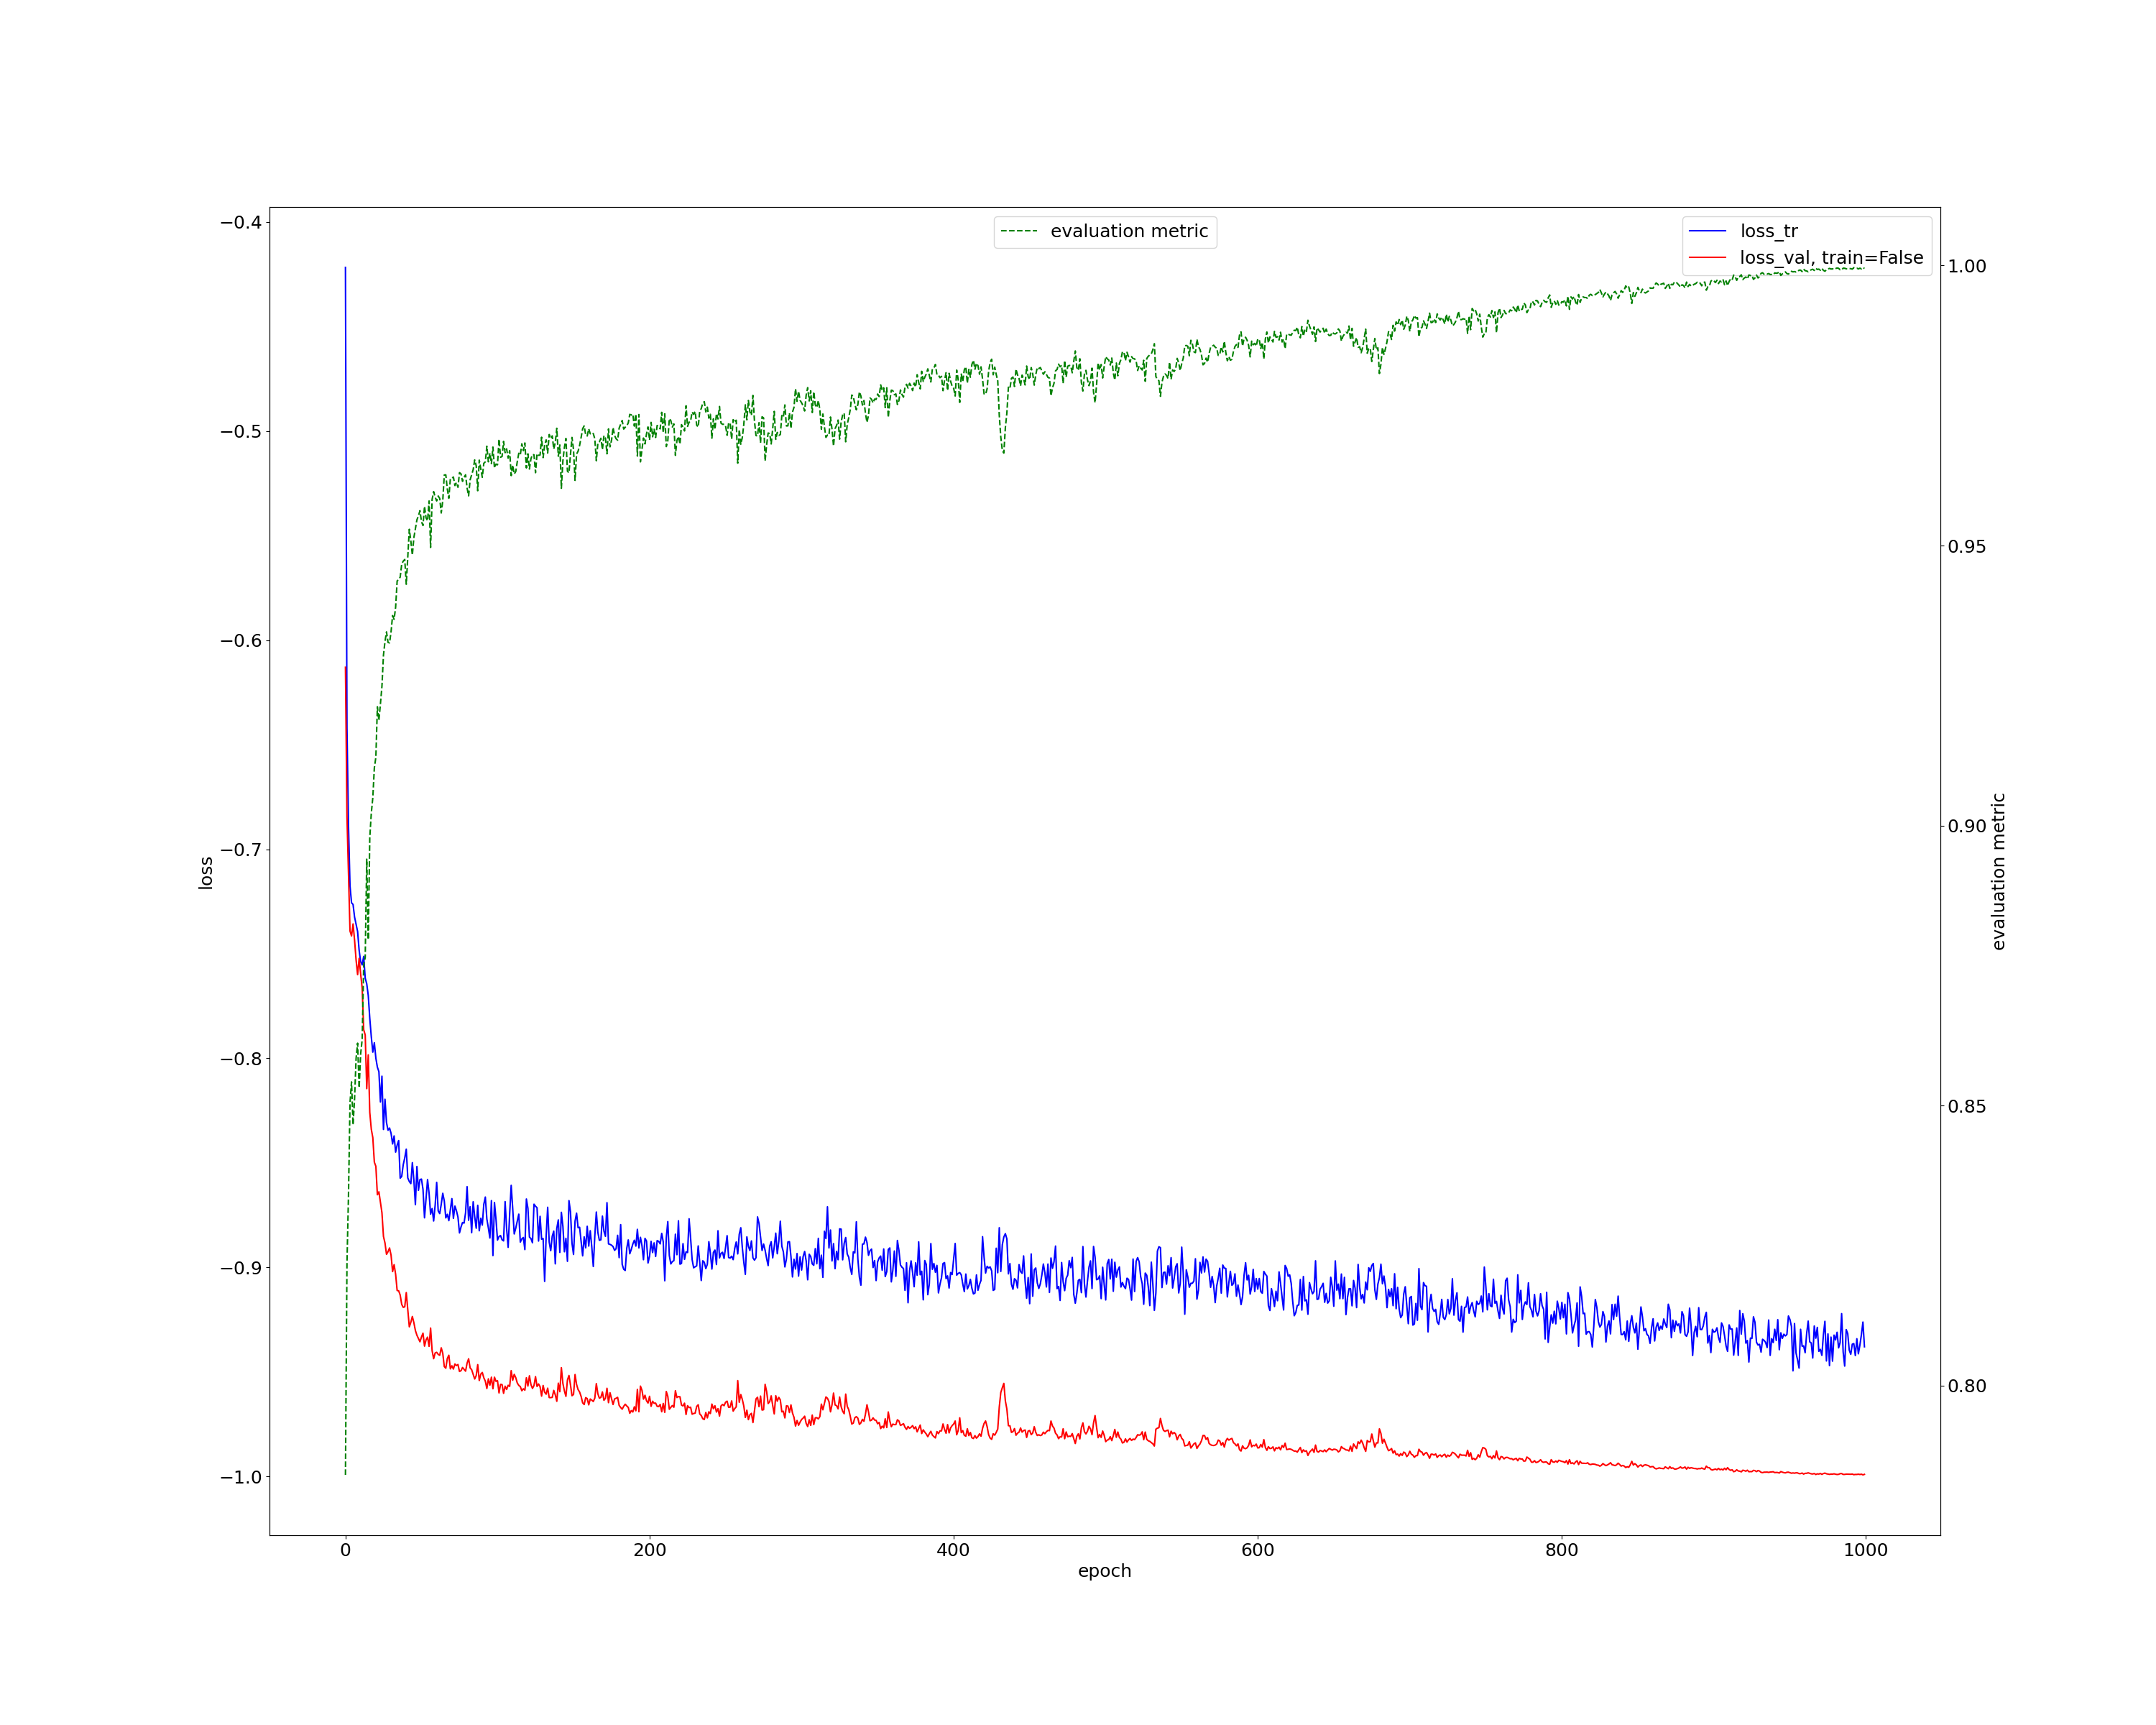
\includegraphics[width=\textwidth]{Pictures/nnUnet/Praxis/Task203-Augen-drittel-testsplit/progress_203-Augen-drittel-split.png}
\caption{Verlauf des Dice-Koeffizienten beim Training über 1000 Epochen}
\label{pic:Prog_203}
\end{subfigure}
\end{minipage}%
\begin{minipage}{.4\textwidth}
\begin{subfigure}{\textwidth}
\includesvg[width=\textwidth]{Pictures/nnUnet/Praxis/Task203-Augen-drittel-testsplit/Scatterplot-Dice-203}
\caption{Scatterplot der Dice-Koeffizienten je Sample für Train- und Testsplit}
\label{pic:Dice_203}
\end{subfigure}
\end{minipage}

\caption{Dice-Koeffizienten zum Retina-2D Datensatz mit einem Drittel als Testsplit}
\end{figure}

Da wir auch hier relativ gute Ergebnisse erzielen konnten, wollten wir das Framework an seine Grenzen bringen und so wenig Trainingsamples wie möglich zur Verfügung stellen. Durch Ausprobieren und schrittweises Annähern haben wir herausgefunden, dass nnUNet, jedenfalls bei diesem Datensatz, mindestens 13 Trainingsbeispiele benötigt, da bei weniger Trainingsbeispielen später beim Training ein \textit{IndexOutOfBounds} Fehler auftritt. Leider ist beim Aufteilen in Train- und Testsplit der Objektanteil in den Samples nicht ganz ausbalanciert, da im Trainsplit nur 11\% der Pixel Adern sind und im Testsplit knapp 12\% (s. Abbildung \ref{pic:Haeuf_205}).


\begin{figure}[H]
\centering
\begin{minipage}{.6\textwidth}
\begin{subfigure}{\textwidth}
\centering
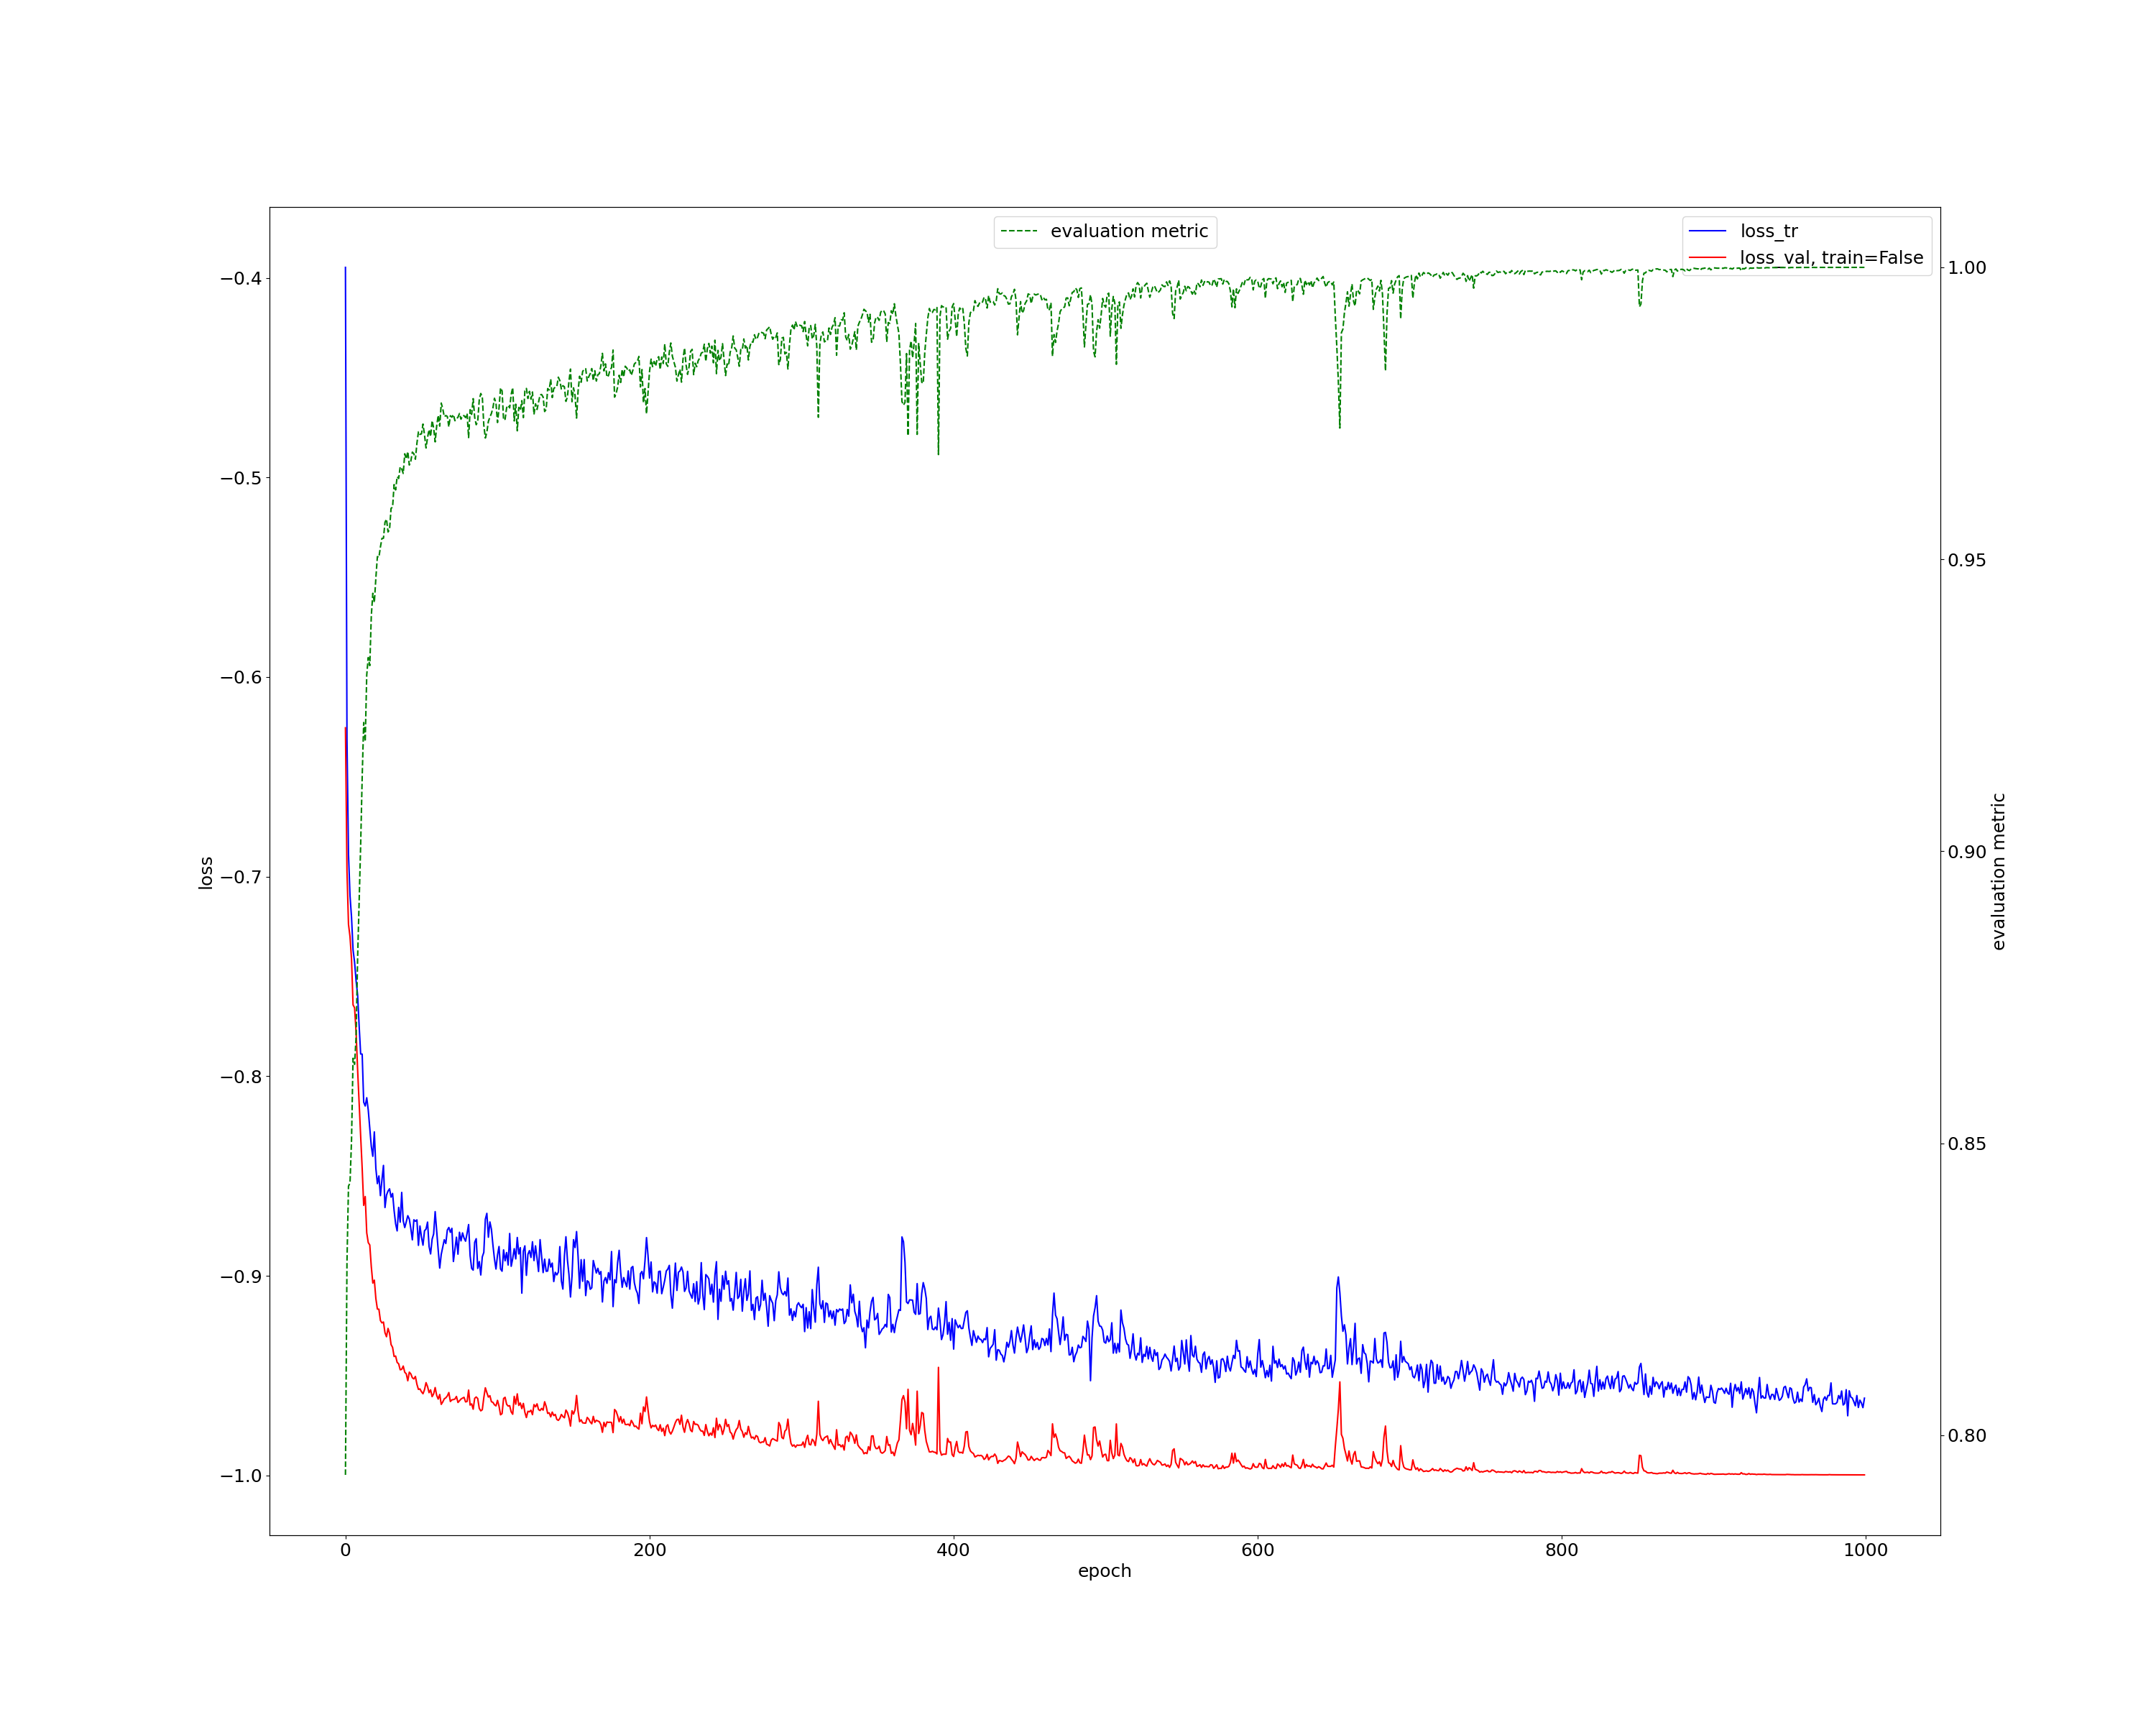
\includegraphics[width=\textwidth]{Pictures/nnUnet/Praxis/Task205-Augen-minimal-13-trainsamples/progress_205-Augen-minimal-13-trainsamples.png}
\caption{Verlauf des Dice-Koeffizienten beim Training über 1000 Epochen}
\label{pic:Prog_205}
\end{subfigure}
\end{minipage}%
\begin{minipage}{.4\textwidth}
\begin{subfigure}{\textwidth}
\includesvg[width=\textwidth]{Pictures/nnUnet/Praxis/Task205-Augen-minimal-13-trainsamples/Scatterplot-Dice-205}
\caption{Scatterplot der Dice-Koeffizienten je Sample für Train- und Testsplit}
\label{pic:Dice_205}
\end{subfigure}
\end{minipage}

\caption{Dice-Koeffizienten zum Retina-2D Datensatz mit einem minimalen Trainsplit von 13 Samples}
\end{figure}


Es fällt auf, dass bei dem minimalen Trainingssplit Overfitting stattfindet, da alle Samples bis auf ein einziges einen Dice-Koeffizienten von genau 1 besitzen (s. Abbildung \ref{pic:Dice_205}). Auch der Progress-Graph (Abbildung \ref{pic:Prog_205}) steigt am Anfang schneller als bei $\frac{2}{3}$ Trainingssplit.\\
Auf dem Testsplit fällt auf, dass bei Durchlauf 1 (Abbildung \ref{pic:Dice_203}) eine Gruppierung stattfindet. Viele Samples liegen sehr nah bei 1 und eine zweite, etwa gleich große Gruppe liegt um $0,85$ herum. Dies kommt sehr wahrscheinlich von unserer, fälschlicherweise durchgeführten, manuellen Data-Augmentation, bei der wir das gleiche Bild mehrmals in rotierter und gespiegelter Form in das Framework gegeben haben. Beim 2. Durchlauf mit minimalem Trainsplit sind die Samples im Testsplit relativ gleichmäßig um den Durchschnitt von $0,83$ verteilt (s. Abbildung \ref{pic:Dice_205}).\\\\
Beim Betrachten der Visualisierung der besten, schlechtesten und mittleren Predictions je Split (Abbildungen \ref{pic:Vis-Train_205}, \ref{pic:Vis-Test_205}) fällt auf, dass die Adern in der Predictions generell breiter sind als in Ground-Truth. Das kommt von der leider notwendigen Verkleinerung der Auflösung der Bilder, da dann bei feinen Adern anstatt nur schwarzer oder weißer Pixel in der Ground-Truth Segmentierung auch graue Pixel entstehen, da z.B. Adern mit einer Breite von einem Pixel nicht weiter in der Auflösung reduziert werden können. Wir haben uns dafür entschieden, die dann grauen Pixel auch als weiße Pixel, also als Ader-Segmentierung, zu zählen, da ansonsten feine Adern Lücken bekommen und die Segmentierung insgesamt schlechter ausfällt. Ansonsten findet man keine groben Fehler, die meisten Adern werden sehr genau erkannt.



\begin{figure}[H]
\centering
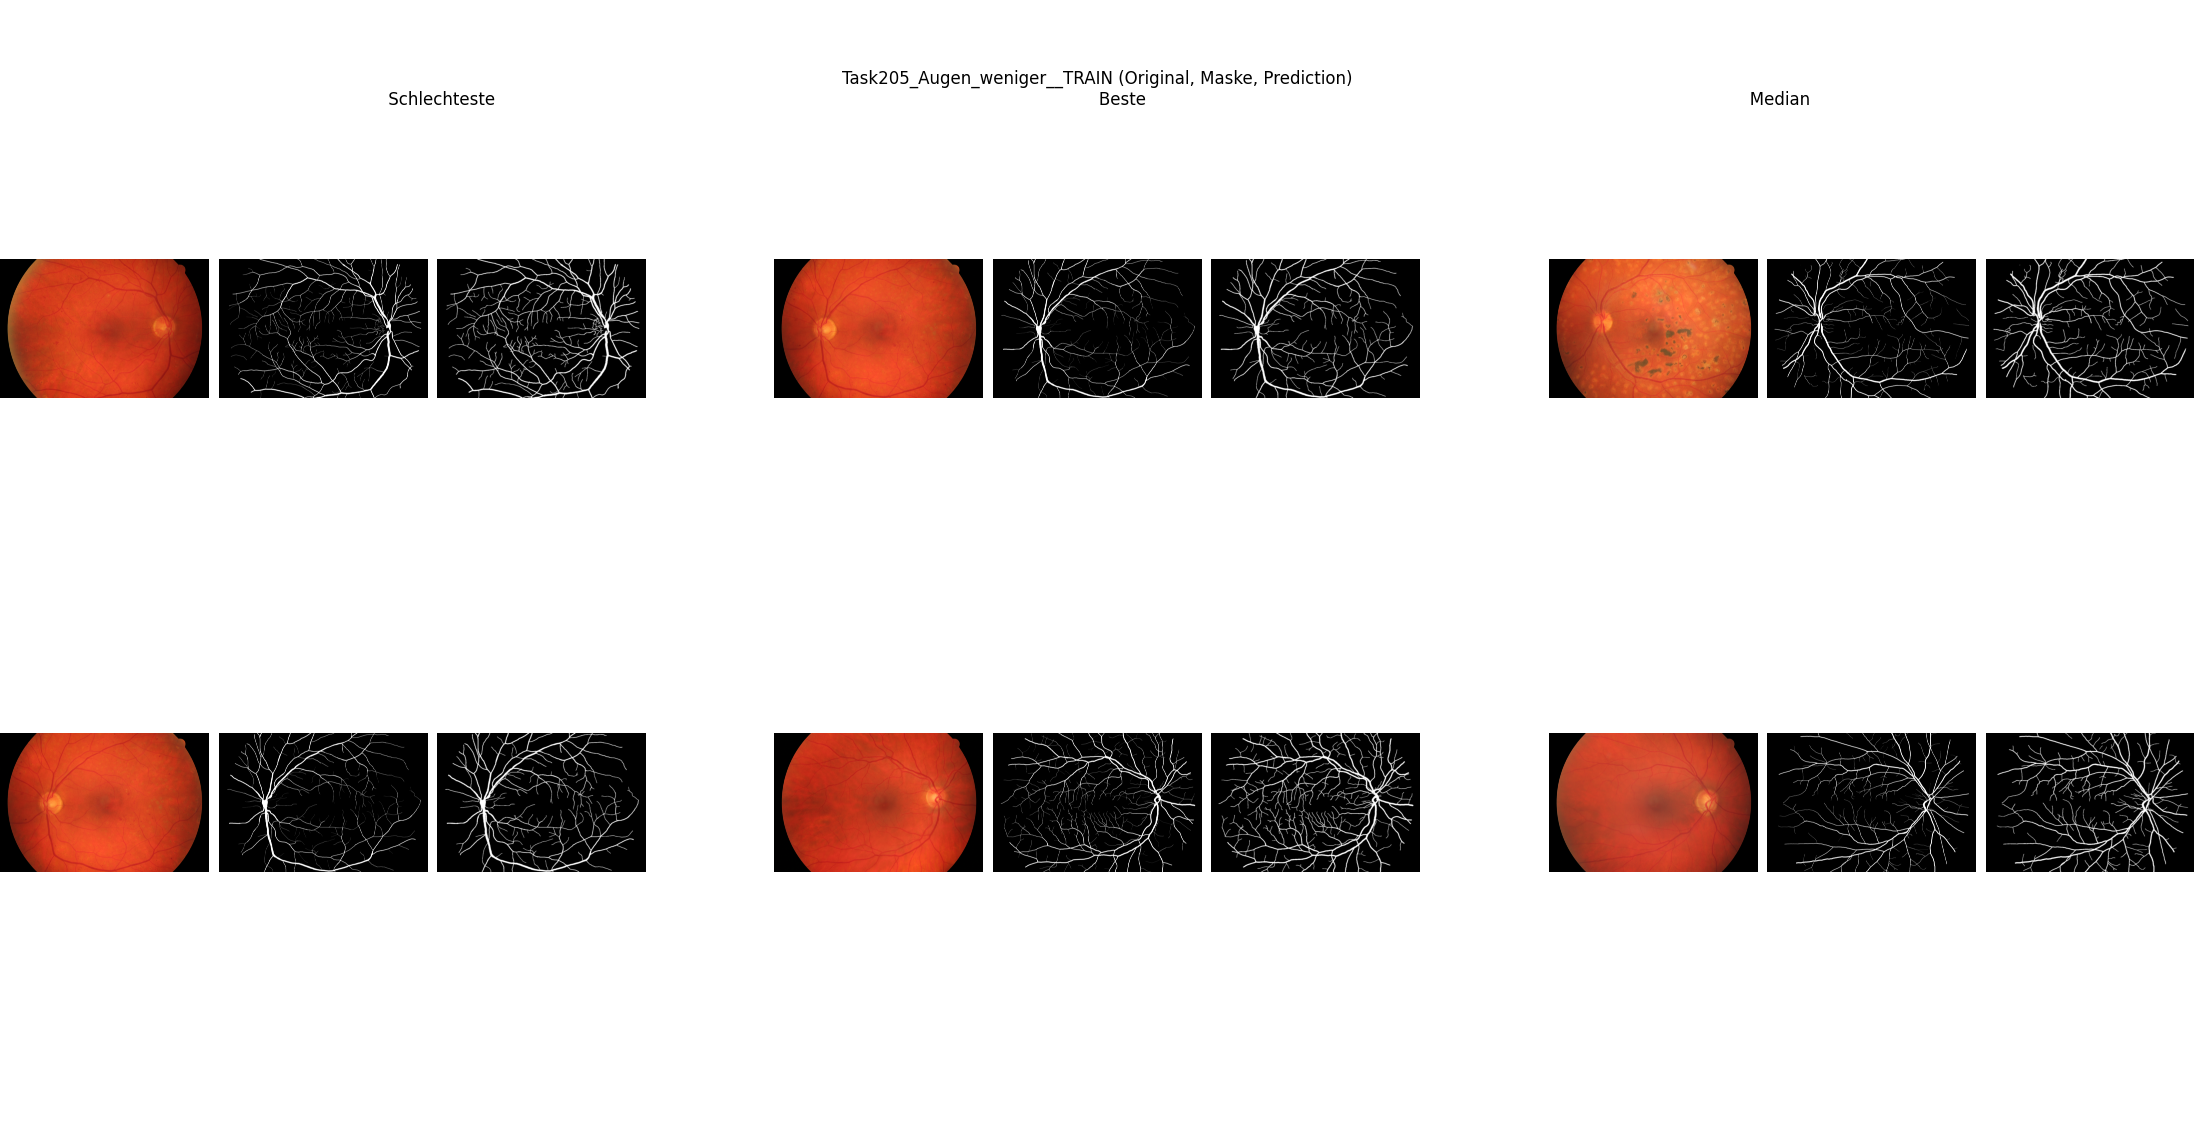
\includegraphics[height=0.35\textheight, width=\textwidth]{Pictures/nnUnet/Praxis/Task205-Augen-minimal-13-trainsamples/Vis-Train.png}
\caption{Visualisierung des Trainsplits auf dem Larvendatensatz mit minimalem Trainsplit (links: schlechteste Ergebnisse, mitte: beste Ergebnisse, rechts: Ergebnisse im Median; jeweils Original, Ground-Truth und Prediction)}
\label{pic:Vis-Train_205}
\end{figure}


\begin{figure}[H]
\centering
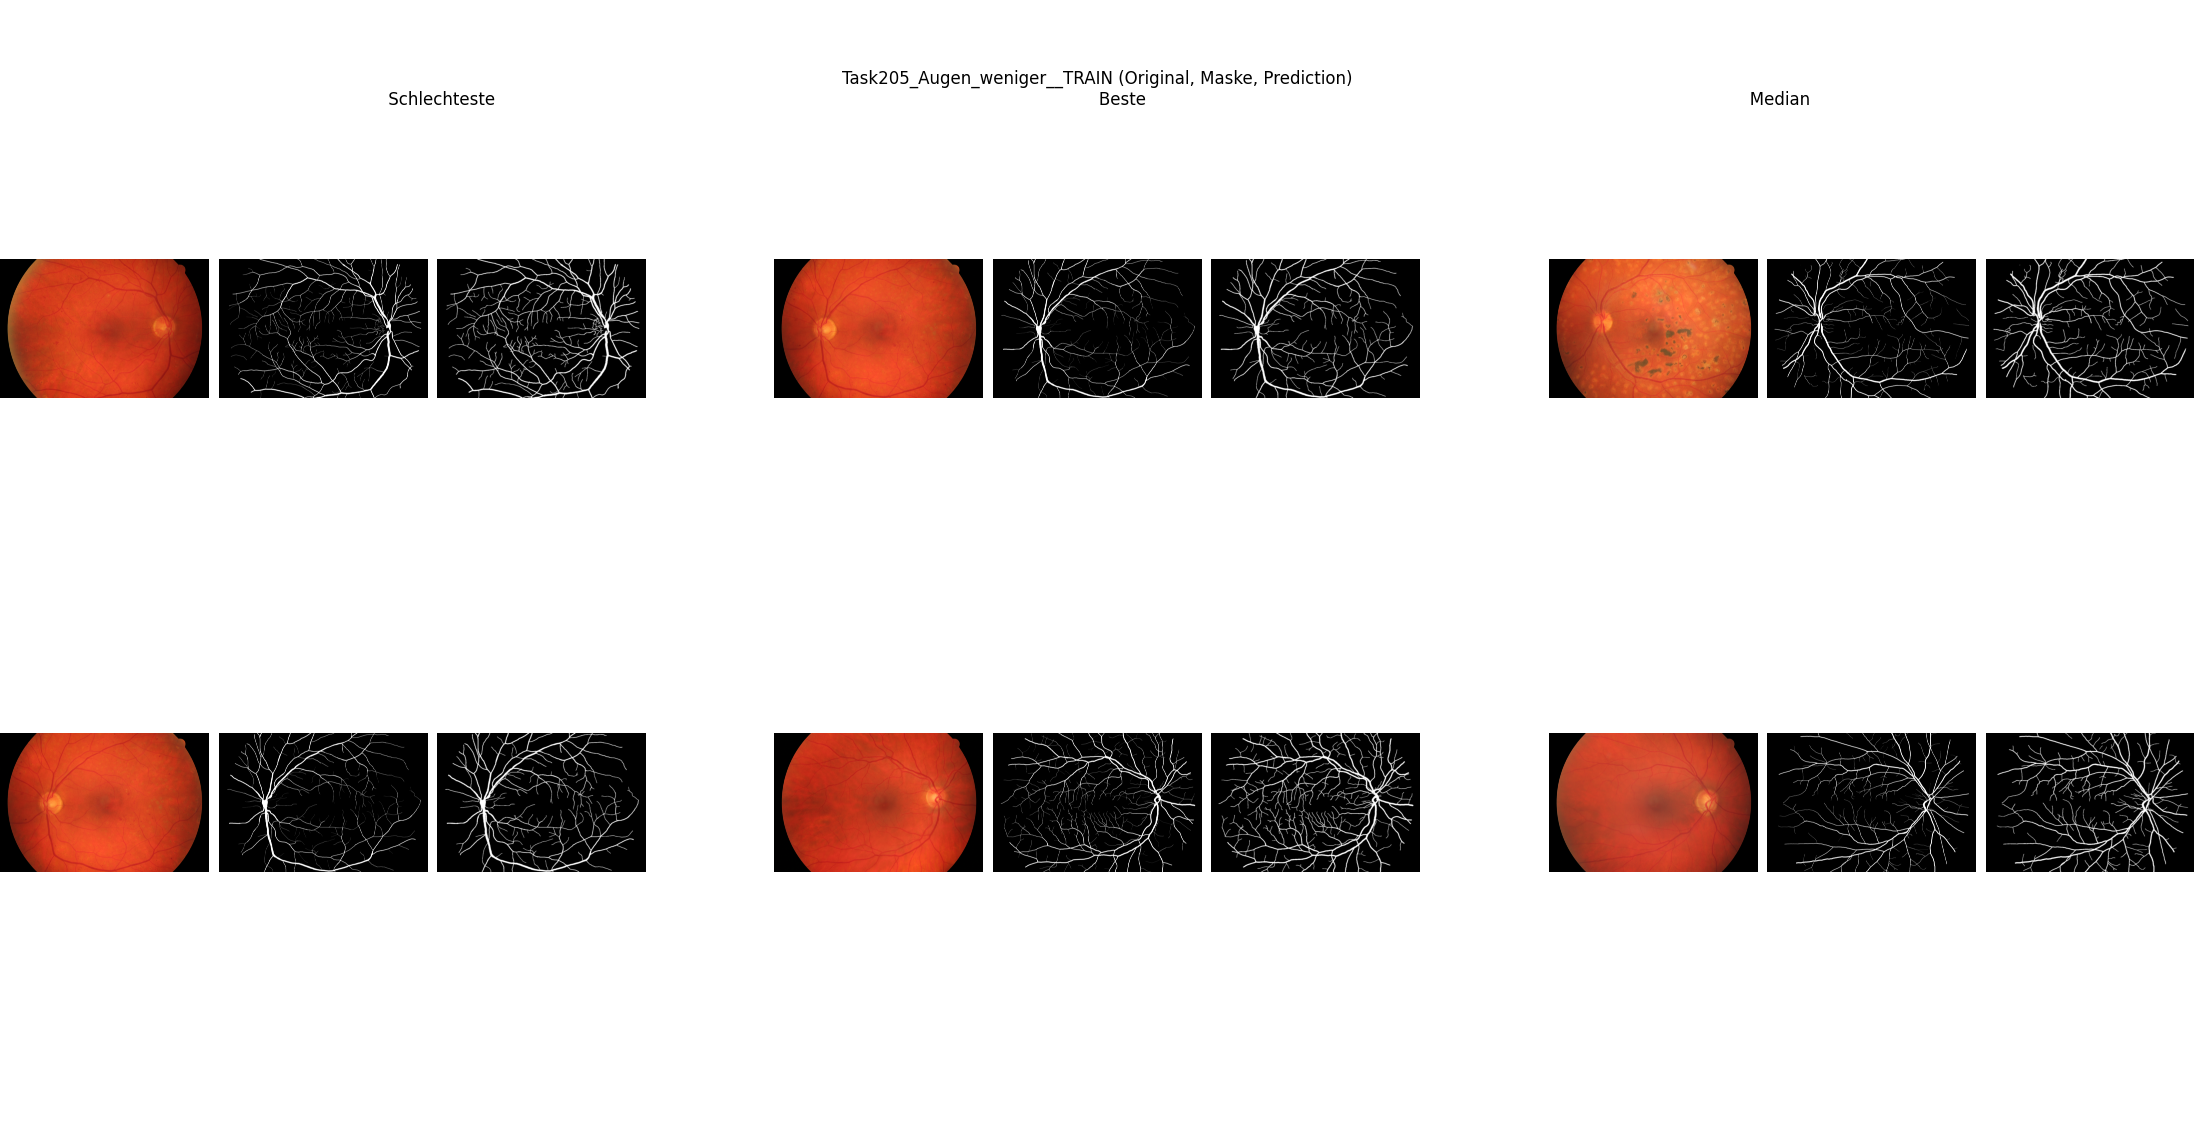
\includegraphics[height=0.35\textheight, width=\textwidth]{Pictures/nnUnet/Praxis/Task205-Augen-minimal-13-trainsamples/Vis-Train.png}
\caption{Visualisierung des Testsplits auf dem Larvendatensatz mit minimalem Trainsplit (links: schlechteste Ergebnisse, mitte: beste Ergebnisse, rechts: Ergebnisse im Median; jeweils Original, Ground-Truth und Prediction)}
\label{pic:Vis-Test_205}
\end{figure}





Da wir bei diesem Datensatz relativ gute Ergebnisse produzieren konnten, haben wir dem Framework komplett fremde Bilder \cite{retina2dExtra} in verschiedenen Auflösungen und Zoom-Stufen zum Segmentieren gegeben. Zu diesen Bildern gab es leider keine Ground-Truth Segmentierung, jedoch kann man auch so grob abschätzen wie robust das Modell ist, und dass es tatsächlich die Merkmale einer Ader in der Retina erlernt hat und sogar mit verschiedenen Auflösungen, Ausschnitten und \textit{Färbungen} der Retina umgehen kann (s. Abbildung \ref{pic:retinaExtraA} und \ref{pic:retinaExtraB}).
\begin{figure}[H]

\begin{minipage}{.5\textwidth}
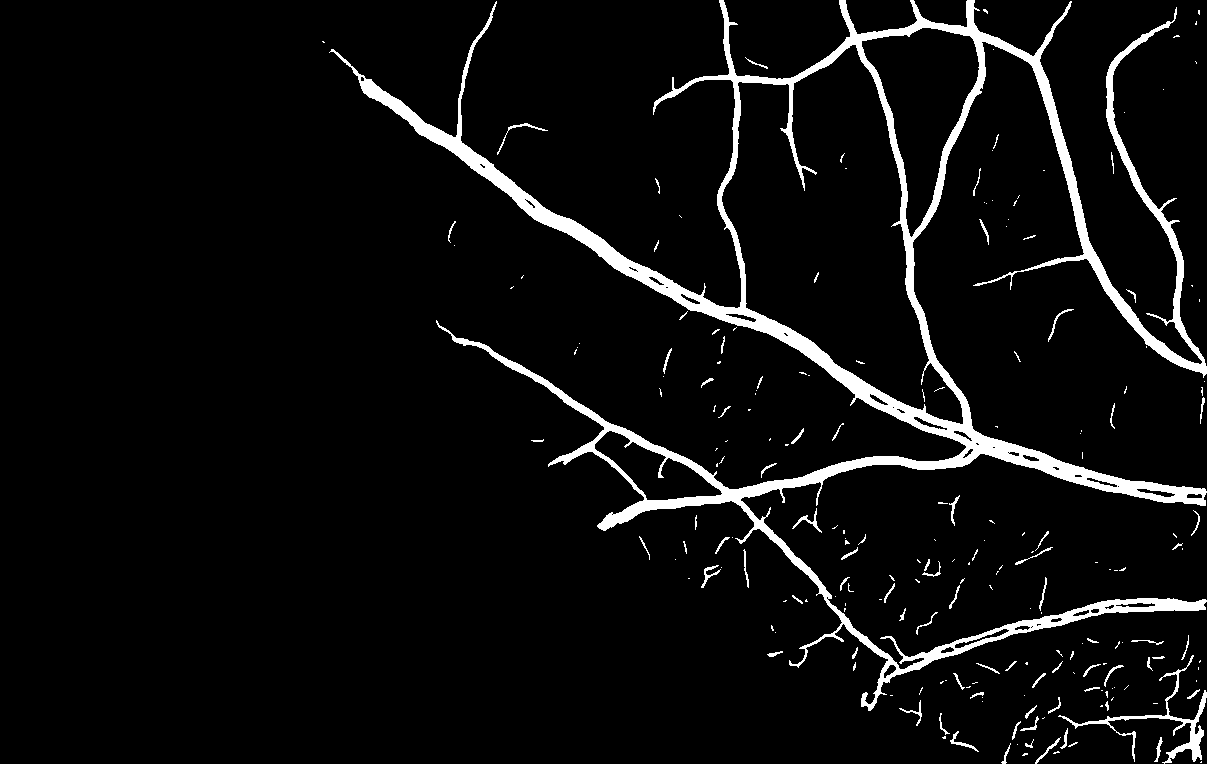
\includegraphics[width=\textwidth]{Pictures/nnUnet/Praxis/Task205-Augen-minimal-13-trainsamples/extra_Bilder/13a_right_cut.png}
\end{minipage}
\begin{minipage}{.5\textwidth}
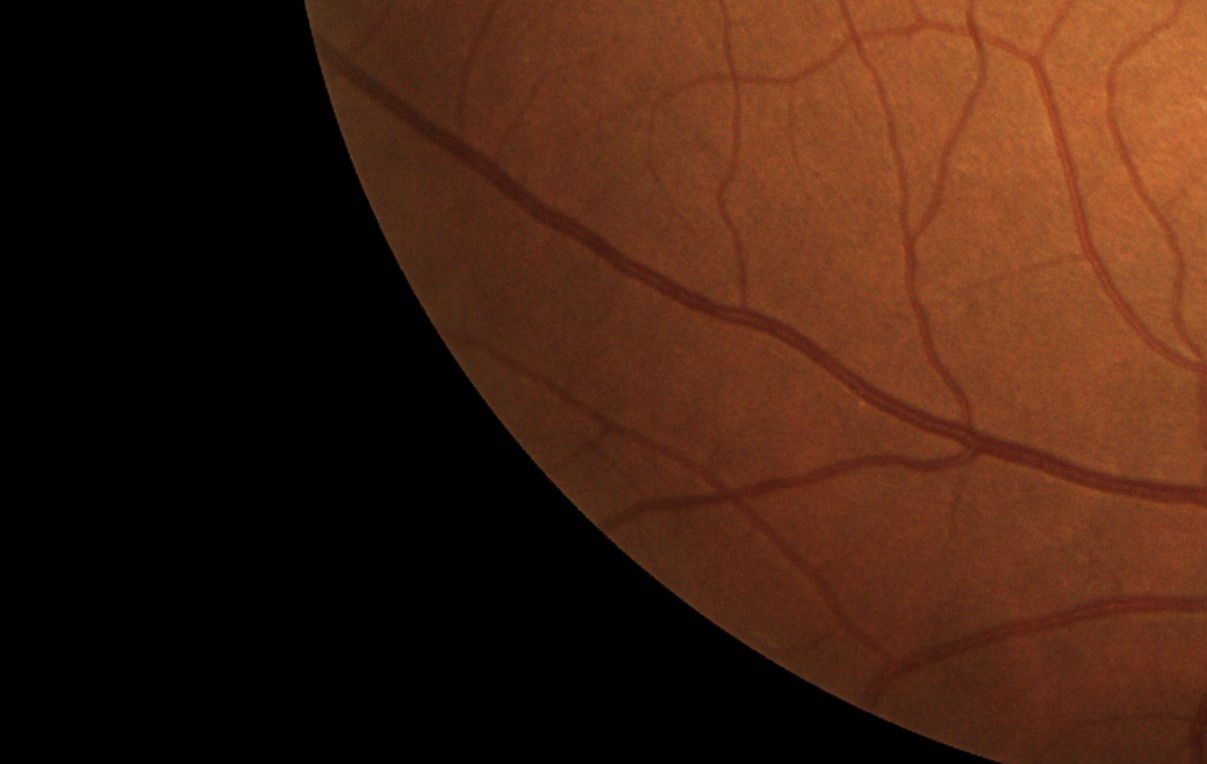
\includegraphics[width=\textwidth]{Pictures/nnUnet/Praxis/Task205-Augen-minimal-13-trainsamples/extra_Bilder/13a_right_cut-original.jpeg}
\end{minipage}
\caption{Bild 13a\_right aus \cite{retina2dExtra} in starkem Zoom - Prediction und Original}
\label{pic:retinaExtraA}
\end{figure}

\begin{figure}[H]
\begin{minipage}{.5\textwidth}
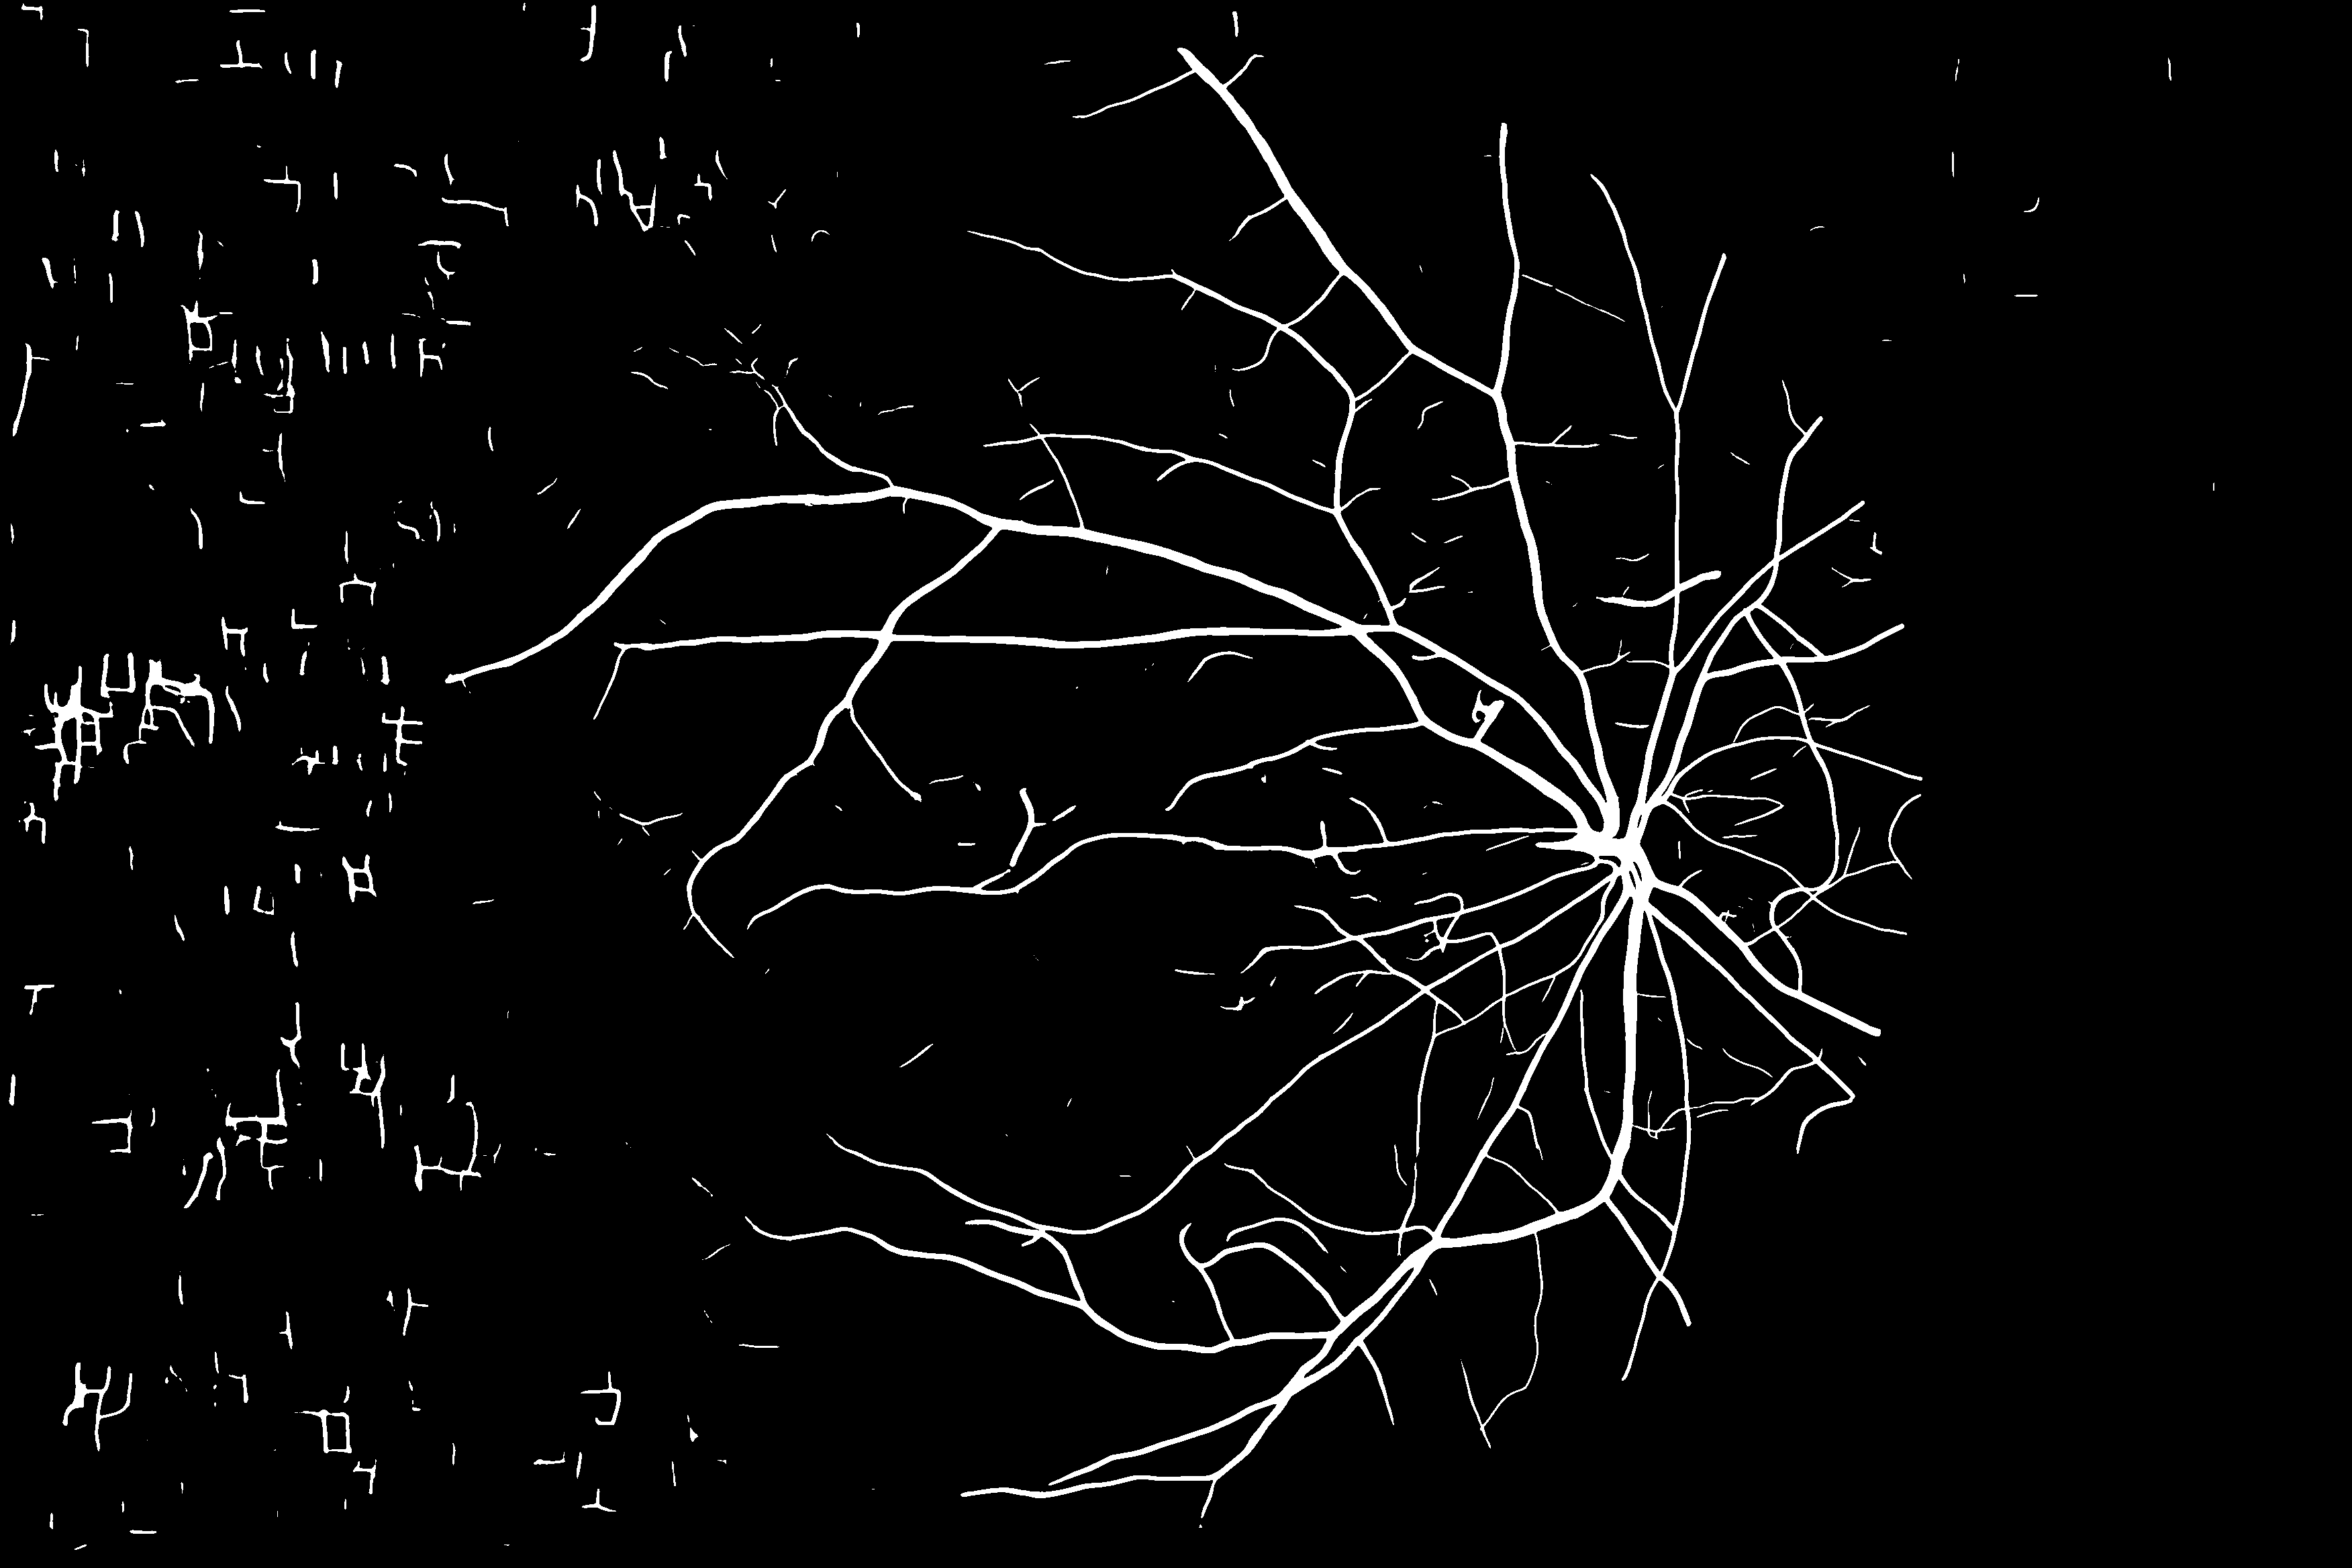
\includegraphics[width=\textwidth]{Pictures/nnUnet/Praxis/Task205-Augen-minimal-13-trainsamples/extra_Bilder/1170_right.png}
\end{minipage}
\begin{minipage}{.5\textwidth}
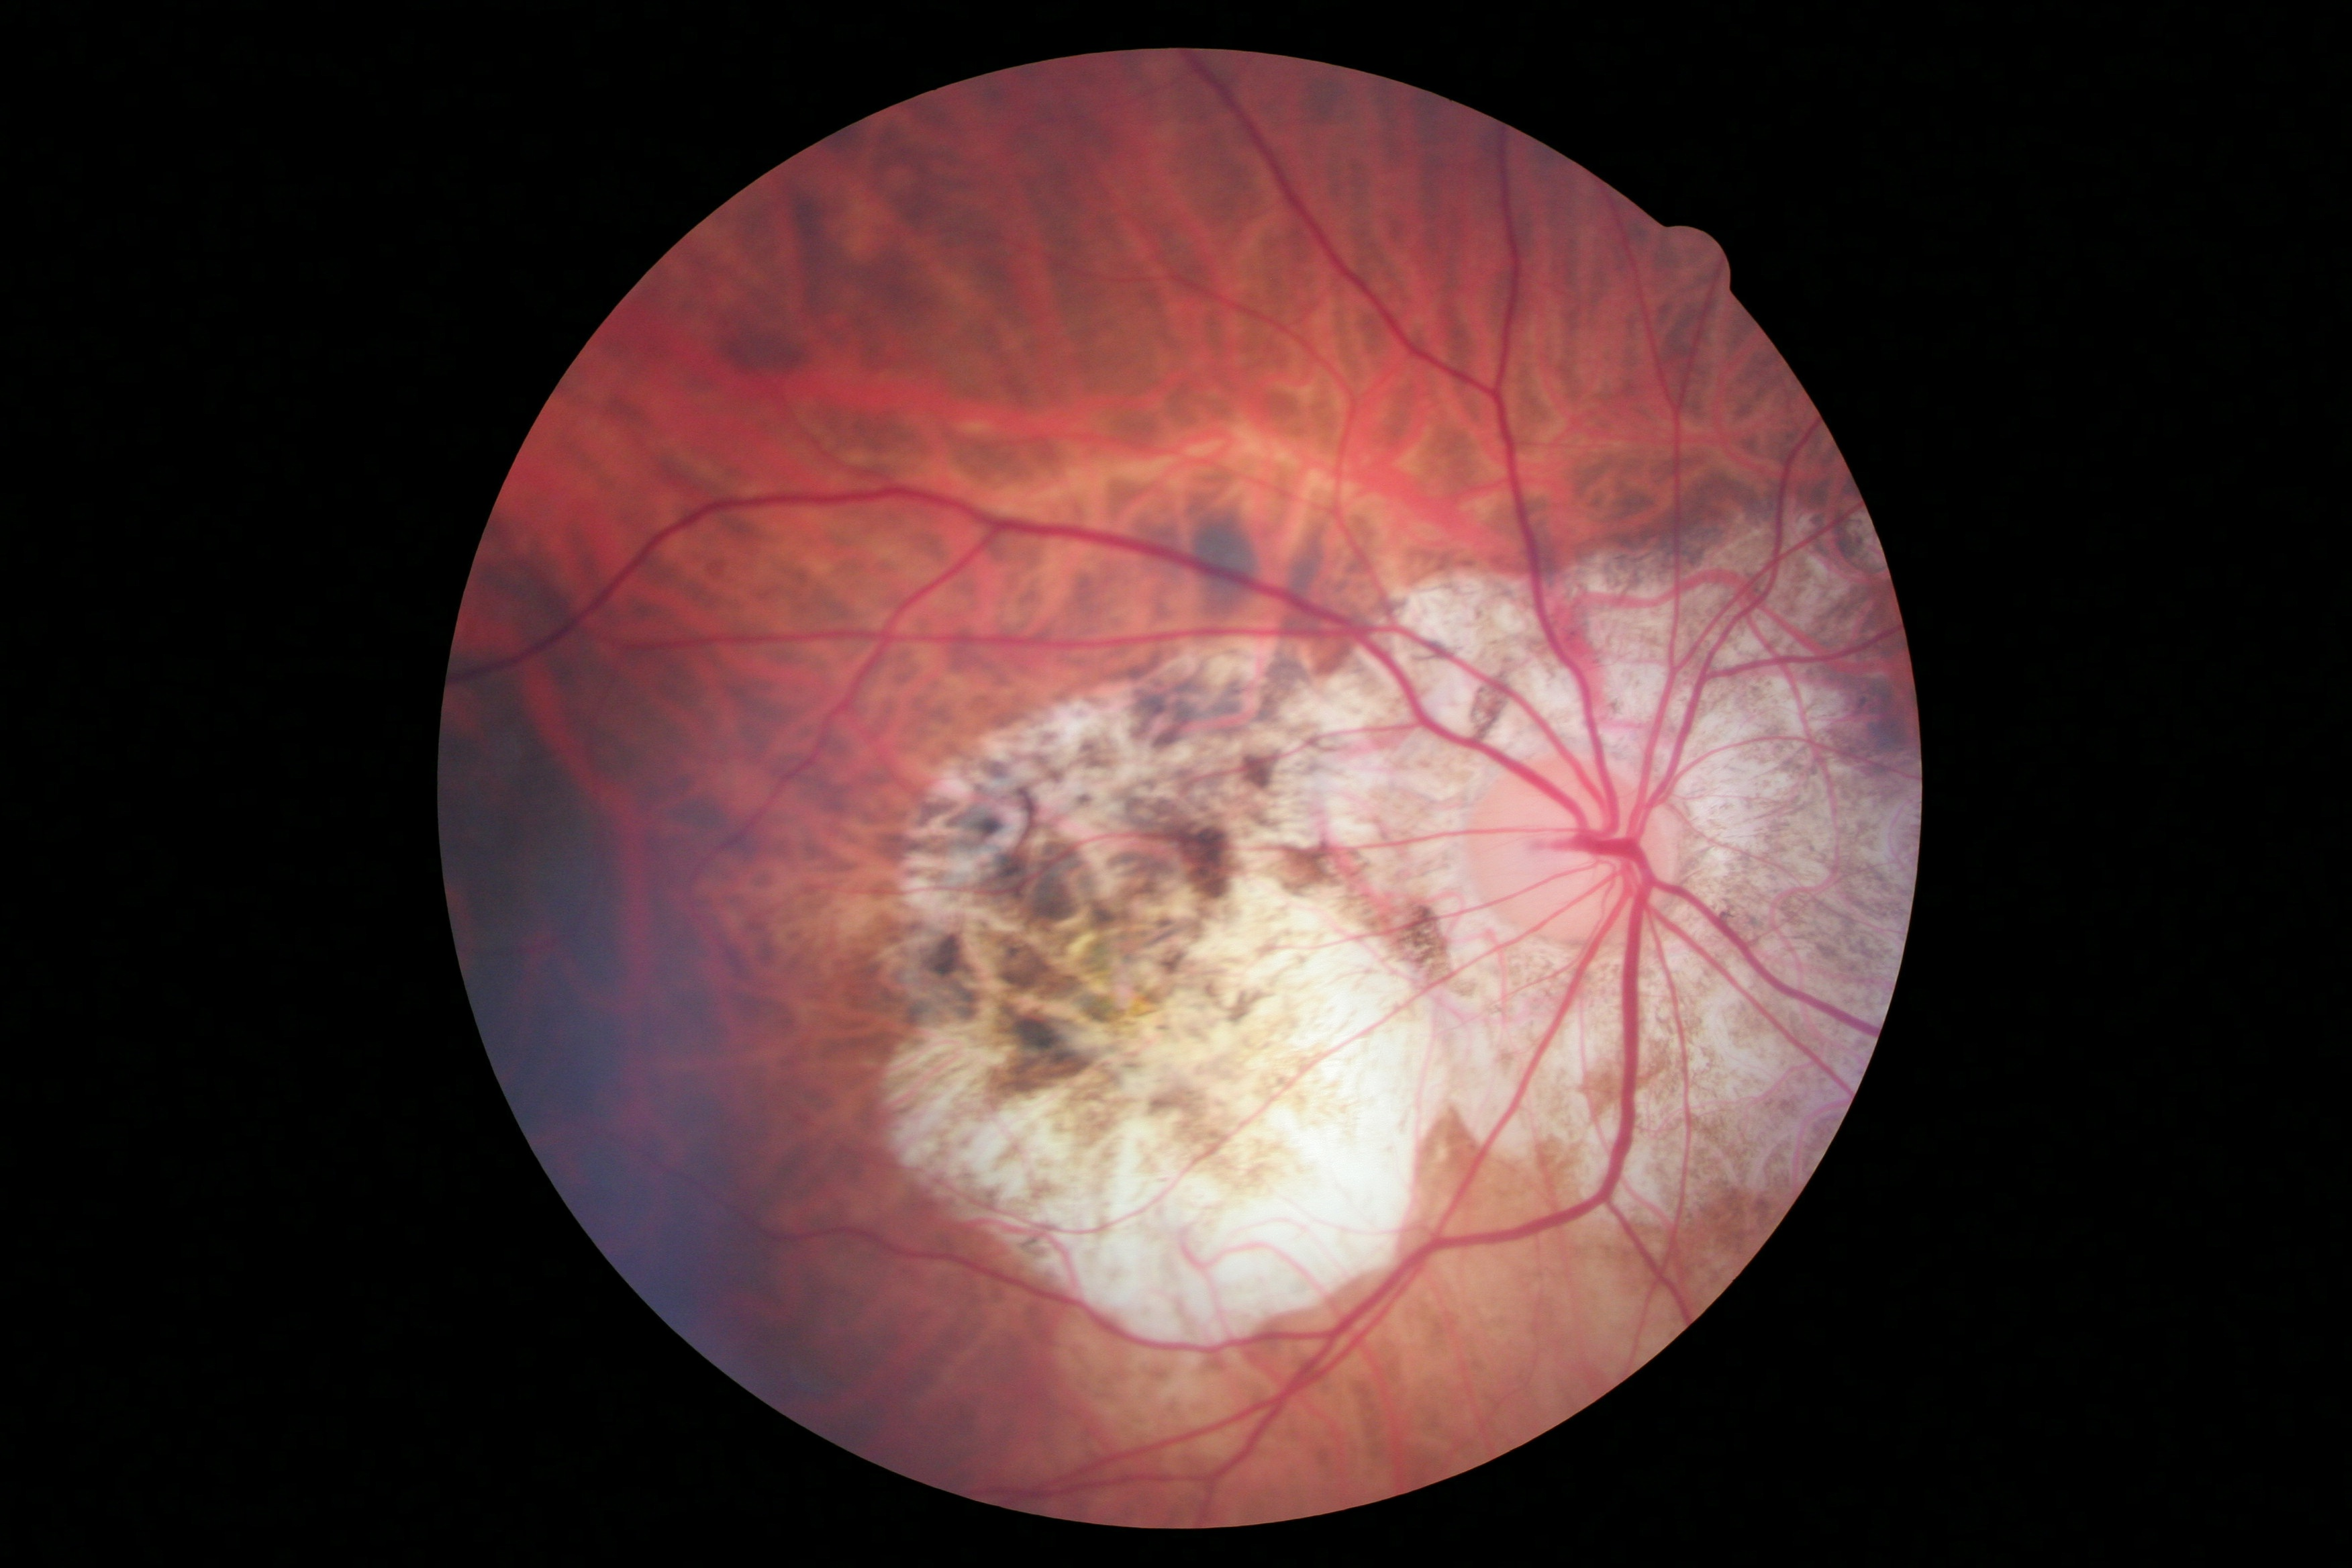
\includegraphics[width=\textwidth]{Pictures/nnUnet/Praxis/Task205-Augen-minimal-13-trainsamples/extra_Bilder/1170_right-original.jpeg}
\end{minipage}
\caption{Bild 1170\_right aus \cite{retina2dExtra} mit Wucherung im Hintergrund - Prediction und Original}
\label{pic:retinaExtraB}
\end{figure}




\subsection{CT-Datensatz}
\todo{Stimmt das so mit dem CT Datensatz?}
Da wir bisher nur eigene 2D-Datensätze in das Framework gegeben haben und es nur wenig öffentlich zugängliche 3D-Datensätze zur Segmentierung gibt, die nicht Teil der MSD-Challenge \cite{msdChallenge} sind, wurde uns ein Datensatz mit 19 Ganzkörper CT-Aufnahmen zur Verfügung gestellt, in denen Kalzium-Ablagerungen am Rand der Gefäße segmentiert werden sollen.
Auffällig ist hierbei, dass trotz der hohen Auflösung des Datensatzes (512x512 mit $\approx$ 400-600 Slices je Sample) nur \textit{sehr} wenig Pixel in der Segmentierung markiert sind. Bestenfalls sind $\approx$ 13000 Pixel im kompletten 3D Volumen bestehend aus 570 Slices mit je einer Auflösung von 512x512, was einem Anteil von \textit{maximal} 0,008\%. Außerdem gibt es auch Samples mit deutlich weniger oder gar keinen markierten Pixeln in der Ground-Truth Segmentierung. \todo{Scatterplot Haeufigkeiten CT} Dies erschwert das Training und könnte eine Begründung für die \todo{\textit{schlecht} gegen etwas angemessenes austauschen} schlechten Ergebnisse sein.\\
Um den Datensatz in nnUNet zu geben mussten wir erst die zur Verfügung gestellten .nrrd (Ground-Truth) und .dcom (3D-CT-Scan) Dateien mit eigenen kleinen Pythonscripten \cite{autoMLGithub} in Nifti-Dateien umwandeln. Beim Trainieren ist uns erst nach zweimaligem Neustarten ohne Erfolg, mit sehr schlechten Ergebnissen bei genauerem Lesen des Papers aufgefallen, dass wir das Preprocessen in nnUNet bisher immer auf dem Login-Node des Clustercomputers Palma II durchgeführt haben, der keine Grafikkarte besitzt, um Wartezeiten in der Warteschlange zu vermeiden. Das Preprocessen ist aber abhängig von den zu dem Zeitpunkt zur Verfügung gestellten Ressourcen, insbesondere des verfügbaren GPU Speichers. Nachdem wir diesen Denkfehler behoben haben und den CT-Datensatz sowohl auf einer GPUv100 Karte preprocessed und trainiert haben, gelang es uns \todo{\textit{einigermaßen akzeptable} ersetzen} einigermaßen akzeptable Ergebnisse zu erzielen. \todo{Verweis auf Visualisierung des CT Datensatzes, Predictions raussuchen und veranschaulichen}
\todo{Verschiedene Versionen diskutieren? 3dcascade, 3dfullres (1000 + 2000) und 2d}

\subsection{Pascal VOC2012}
\todo{Gewichtung für Average als Formel darstellen}
Nachdem wir bei den bisherigen 2D-Datensätzen nur Graustufen-Bilder mit einer Klasse (Larven) und farbige Bilder mit einer Klasse (Retina 2D) verwendet haben wollten wir auch noch einen 2D-Datensatz in Farbe mit mehreren Objekt-Klassen ausprobieren. Die Entscheidung fiel relativ schnell auf Pascal VOC2012 \cite{PascalVOCDatensatz}, da dieser sehr viele Klassen (20 Klassen + Background) und viele segmentierte Bilder (2856 Stück) in verschiedenen Formaten und Auflösungen zur Verfügung stellt und von vielen anderen Frameworks zum Vergleichen verwendet wird. Außerdem ist dieser Datensatz mit Fotografien nochmal wesentlich weiter von der \enquote{biomedical-domain} \cite{nnunetGithub2D-Daten}, für die das Framework eigentlich erstellt wurde, entfernt und dient somit als Test, wie robust das Framework mit verschiedenen Daten umgeht.\\\\
Um die Pascal-VOC 2012 Bilder in nnUNet zu geben mussten erst die Farbkodierungen in der Ground-Truth-Segmentierung in Indizes umgewandelt werden \cite{autoMLGithub}, da nnUNet bei 0=Background beginnend aufsteigende Integer für die Klassen erwartet aber in dem Pascal-Datensatz \cite{PascalVOCDatensatz} die Segmentierung zur besseren Erkennbarkeit farblich gekennzeichnet ist.\\
Außerdem mussten 57 Bilder, die nicht farbig sondern nur in Graustufen in Pascal-VOC 2012 \cite{PascalVOCDatensatz} vorhanden sind entfernt werden, da das Framework nicht mit einer variablen Anzahl an (Farb-) Kanälen umgehen kann.\\\\

Bei der Auswertung ist uns aufgefallen, dass die Accuracy (Dice) zwischen den verschiedenen Klassen stark schwankt und das Framework manche Klassen deutlich besser erkennt als andere. \todo{Ergebnisse ausformulieren, Bilder einfügen}

\subsection{Retina 3D-Datensatz}
Abschließend haben wir, da wir auf dem anderen 3D-Datensatz mit CT-Aufnahmen \todo{anders formulieren, Ergebnisse sind halbwegs ok} keine guten Ergebnisse erzielen konnten, einen weiteren 3D-Datensatz mit Retinae zur Verfügung gestellt bekommen. Er besteht aus 21 Samples von 3D-Scans der Retina mit Segmentierungen. Diese Samples liegen sowohl in ihrer ursprünglichen, gekrümmten Form vor als auch in einer geplätteten Form, die die Krümmung der Netzhaut heraus rechnet. Wir haben uns auf die gekrümmte Version beschränkt.\\\\
Wir haben wieder die zur Verfügung gestellten .mat Dateien in Niftis konvertiert \cite{autoMLGithub} und das Training gestartet.
\todo{Ergebnisse einfügen, diskutieren wie 3d\_fullres und 2d sich unterscheiden, Ensemble auch}





\section{Fazit}
Besonders gut gefallen hat uns der einfache Umgang mit dem Framework. Alle Schritte sowohl zur Installation als auch zum Umgang mit neuen und eigenen Datensätzen wurden detailliert in einer Anleitung erklärt und auch der Code ist sehr gut dokumentiert, was zum Verständnis deutlich beiträgt \cite{nnunetGithub}.\\
Das Framework machte von Anfang an einen durchdachten, anwenderfreundlichen Eindruck. Die Bedienung ist ziemlich einfach und das Framework nimmt dem Anwender jegliche Arbeit ab, so wie es sein sollte.
\todo{Guter Support: Github Issue Antwortzeit nur wenige Tage, schnelle bugfixes}
\todo{Die anderen beiden Frameworks kritisieren, dieses ist deutlich besser / das einzige was überhaupt funktioniert...}


% Fazit

%!TEX root = ../AutoML-fuer-Segmentierung.tex
\chapter{Gesamtfazit}
\label{ch:conclusion}

%Hier kann beliebig \section{} gesetzt werden


% Einträge in die ToDo-Liste setzen (für Änderungen muss 2 mal übersetzt werden, wie bei TOC auch)
\todo{Fazit mit Inhalt füllen}






\appendix % hier beginnt der Anhang
%%!TEX root = ../AutoML-fuer-Segmentierung.tex
\chapter{Ein Anhangskapitel}

%Hier kann beliebig \section{} gesetzt werden

% Einträge in die ToDo-Liste setzen (für Änderungen muss 2 mal übersetzt werden, wie bei TOC auch)

% Literaturverzeichnis (Referenzen der Zitate) ausgeben
\printbibliography

\end{document}
